\documentclass[12pt, a4paper]{scrreprt}

\renewcommand*\familydefault{\sfdefault} 
%\usepackage[T1]{fontenc}

\usepackage[english]{babel}
%\usepackage{cite}
\usepackage[utf8]{inputenc}
%\usepackage[onehalfspacing]{setspace}
\usepackage{geometry, textcomp}
\newgeometry{right=2cm,left=4cm, top=2.5cm, bottom=2.3cm, footnotesep=0.5cm}
%\usepackage[acronym]{glossaries}

\usepackage[printonlyused]{acronym}  % Abkürzungsverzeichnis [nur verwendete Abkürzugen]

%\glsenablehyper

%\makeglossaries

\usepackage{savesym}
\usepackage{amsmath,amssymb,amstext}
%\usepackage{graphics}
\savesymbol{iint}
\usepackage{txfonts}

\restoresymbol{TXF}{iint}
\usepackage[automark,headsepline,ilines,komastyle]{scrpage2}
\usepackage{blindtext}
\usepackage[euler]{textgreek}
\setlength{\parindent}{0pt}
\setlength{\headheight}{1.5\baselineskip}
\renewcommand{\baselinestretch}{1.5}

\pagestyle{scrheadings}
\clearscrheadfoot
\ihead[]{}
\chead[]{}
\ohead[]{\headmark \hfill \thepage}
\ifoot[]{}
\cfoot[]{}
\ofoot[]{}

\setheadsepline[\textwidth]{1pt}
\usepackage{tabularx}
\usepackage{colortbl}
\usepackage{multirow}
\usepackage{hhline}
\usepackage{array}
\usepackage{tocloft}
\usepackage[hidelinks]{hyperref}
\tocloftpagestyle{scrheadings}
\renewcommand{\chapterpagestyle}{scrheadings}
\usepackage[font=footnotesize]{caption}

\usepackage{tikz}
\usepackage{rotating} 

\newenvironment{packed_item}
	{\begin{itemize}
			\setlength{\itemsep}{0pt}
			\setlength{\topsep}{0pt}
			\setlength{\parsep}{0pt}
			\setlength{\parskip}{0pt}}
		{\end{itemize}}
	
\usepackage[style=authoryear, natbib=true, backend=biber]{biblatex}

\renewcommand{\nameyeardelim}{ }
\usepackage[babel,german=guillemets]{csquotes}

\makeatletter

\newrobustcmd*{\parentexttrack}[1]{%
	\begingroup
	\blx@blxinit
	\blx@setsfcodes
	\blx@bibopenparen#1\blx@bibcloseparen
	\endgroup}

\AtEveryCite{%
	\let\parentext=\parentexttrack%
	\let\bibopenparen=\bibopenbracket%
	\let\bibcloseparen=\bibclosebracket}

\makeatother

\usepackage{pstricks}
\usepackage{pstricks-add}

\bibliography{Lit.bib}

\usepackage[final]{pdfpages}

\begin{document}
		\begin{titlepage}
			\begin{center}
			%\setlength{\headheight}{1.5\baselineskip}
			\renewcommand{\baselinestretch}{1.5}
					\textbf{\large FOM - Hochschule für Oekonomie \& Management \\
						Hamburg \\
						\ \\
						Master-Studiengang Big Data \& Business Analytics \\
						3. Semester \\
						\ \\
						Development of a system to control and monitor blood pressure \ \\
						measurements to prevent cardiovascular disease \ \\
						\ \\
						}
						
					\textrm{
						\ \\
						Betreuer: Prof. Dr. Kai Brüssau \\
						\ \\
						Autor: Jacqueline Franßen \\
						\ \\
						Matrikel-Nr: 496804 \\
						\ \\
						3. Fachsemester \\
						\ \\
						Hamburg, den 29.02.2020 \\
						}
			\end{center}
		\end{titlepage}

%\includepdf{Image/Deckblatt.pdf}

			\setcounter{tocdepth}{3}
			\setcounter{secnumdepth}{3}		
			\pagenumbering{Roman}
			\thispagestyle{empty}
			\pdfbookmark{\contentsname}{toc}\tableofcontents
			\newpage
			\listoffigures
			\listoftables

			\pagenumbering{arabic}
			\thispagestyle{empty}
\chapter{Abstract}\label{abstract}

This scientific article focusses on the development of a chatbot and the analysis of blood pressure measurements.
The main purpose of this scientific article is to develop a chatbot that reminds patients of their measurements, since in the past, many patients tended to forget their measurements or did not measure precisely. This can lead to severe cardiovascular disease. By developing an intent model which focusses on various typical scenarios, patients and doctors should be warned if there are negative trends in the blood pressure values. What is more, patients should be motivated to a more precise measurement by human-like conversations.
Besides, developed system can be divided into four major business cases. 
The first business case is that doctors can get an overview of the patient's blood pressure values. It enables them to react more precisely to any special values or trends.
Second, the measurements are taken more accurately since the patient is lead by a chatbot through a tutorial. Furthermore, the chatbot reminds the patient of his regular measurement, controls and analyses the measured values. As a consequence, it improves the process of documentation.
Third, doctors are informed in-time when there are outliers because a service sends a report regularly via email. Consequently, doctors are able to interprete the values faster.
Fourth, patients get a recommendation of the nearest doctor which helps them to keep their appointments.
Last, a neural network was developed to calculate the probability of suffering from cardiovascular disease of a patient. This information can be useful for the doctor as well as the patient to prevent the break out of the disease.

\chapter{Introduction}\label{introduction}

\section{Problem statement}
According to the organization Deutsche Hochdruckliga \footnote{cf.\autocite{hochdruckliga}}, hypertension is one of the most common disease in our today's society. It can lead to cardiovascular disease and has many different curses, such as false nutrition, overweight or little movement.
Another problem are the measurements, taken by patients at their home. Often, hypertension patients do not measure their blood pressure regularly or forget to write down their measured values. 
What is more, the treating doctors often get a large list of measured values (pulse, systolic and diastolic values) which they have to interprete in short-term. Often, the diagnosis or treatment and medication of these doctors depends on the average value or minimum and maximum value which was measured. 
All of these use cases can be automated and implemented by an application to prevent cardiovascular disease. The next section will explain the aims of this work and how they were implemented.

\section{Aim and scope of this work}
The first aim of this scientific work is to develop a solution to document blood pressure in order to react preventively against heart disease.
To recommend an appropriate doctor in one's surrounding (approximately 5 kilometers of distance), an intuitive user interface with map is being shown.
The application shall send a weekly report (including a diagramm of all measured blood pressure values of the patient) to the doctor so that the doctor will be informed in real-time. In the frontend, it is possible to select different scales on the diagrams, e.g. like the values of last week, month or year. 
At the beginning of using the Chatbot, the user is being led through a tutorial which shows him how to measure his blood pressure correctly. One instruction is for example not to drink coffee before measuring the blood pressure or to sit for at least 5 minutes. After that, a routine for the measurement leads the patient through the measurement. The measured values are saved automatically into a \ac{json} file.
In order to build up diagrams and the neural network that calculates the probability of cardiovascular disease, a sample dataset from Kaggle was used. But for future use cases, it would be better, to have real data from patients interacting with the chatbot. The whole analytics process and implementation will be explained in section \ref{predict}. What is important, the developed model is only a reference model and can be improved by changing the parameters and using real test data. Moreover, in order to get a precise diagnosis of any disease (in this case cardiovascular disease) which depends on many factors (e.g. the appearance of the patient), the advice and treatment of a real doctor should be taken.

\chapter{Fundamentals}\label{fundamentals}

\section{Software Architecture: Best Practices}

In this section, the 'best practices' of software architecture are described. To give an example, the architecture of a blockchain \ac{p2p} network which is backed with a distributed ledger system (see figure \ref{example_software_architecture}) will be explained. According to the authors, Talukder et al.\footnote{cf.\autocite{talukder} pp.258}, the model is an appropriate solution for health applications because they support multiple stakeholders. This fact can be useful for the development of multiple users which all have their proper dashboard (e.g. a doctor's dashboard vs. a patient's dashboard).

\subsection{\ac{soa} for big data applications in the cloud}
The state-of-the-art architecture for any project is \ac{soa} and has many advantages, such as flexibility, agility, process orientation, time-to-market and innovation\footnote{cf.\autocite{zimmermann} pp.130}. What is more, \ac{soa} is convenient for cloud computing since it is ready for extended service models.
Figure \ref{esarc_example} shows the architecture 'ESARC', developed by Zimmermann et al.\footnote{cf.\autocite{zimmermann} p.132}. It helps to cluster, classify, examine, compare, evaluate quality and optimize enterprise architectures. As depicted by figure \ref{esarc_example}, there is a link between enterprise and business information and design for supporting strategic initiatives. What is more, ESARC enables integration capacities for \ac{it} management, software engineering, service and operations management as well as process improvement initiatives.

\begin{figure}[h!]
	\centering
	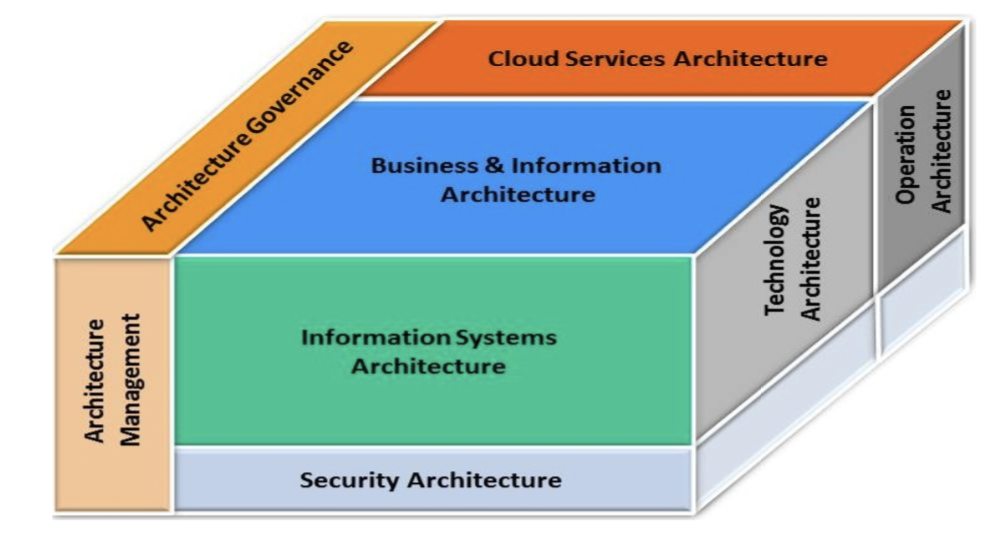
\includegraphics[width=1\textwidth]{images/esarc_cube.png}
	\caption{\ac{esarc} as an example for big data architecture cf.\autocite{zimmermann} pp.133}
	\label{esarc_example}
\end{figure}

As can be seen in figure \ref{esarc_example}, metamodels are used to define model elements in architectures. They relate architectural elements to ontologies which represent a common vocabulary for enterprise architectures.
Zimmermann et al. recommend that operations of tasks and entity services should not have any knowledge about their process or interactive usage context \footnote{cf.\autocite{zimmermann} pp.133}. Instead, task service operations should be independent from users and sessions and should only implement business functionality.

\begin{figure}[h!]
	\centering
	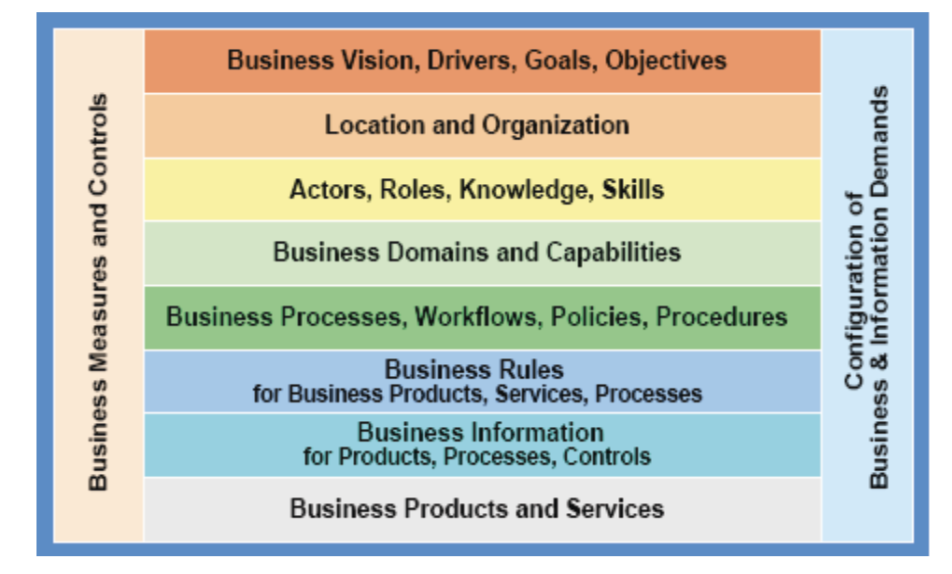
\includegraphics[width=1\textwidth]{images/esarc_business.png}
	\caption{\ac{esarc} business and information reference architecture cf.\autocite{zimmermann} pp.134}
	\label{vp_architecture}
\end{figure}

Figure \ref{vp_architecture} shows a more detailed view of 'ESARC', the procedural framework for architecture assessment processes and questionnaire design. On top of the graphic, with orange background, there are business vision, drivers, goals and objectives. To be more precuse, architecture governance has the goal to manage activities such as plan, define, enable, measure, control and sets rules for architecture complicance to internal and external standards. 

\paragraph{Actors in cloud computing}
According to Zimmermann et al., the main actors in cloud computing are cloud consumers, providers, auditors and broker. In general, all \ac{soa} services are cloud services and follow a reference architecture: 'Jericho-Security-focused Service-oriented Reference architecture for cloud computing'. Thereby, management perspectives from \ac{itil} and \ac{togaf} standards are integrated.

\subsection{Data mining in medical context}

As a common problem in every big data project, there are multiple data sources and systems which provide relevant information for the particular use case. Generally, three types of data sources can be distinguished: For instance, the information can be handwritten human readable and human understandable medical notes. Besides, some information are computer readable and human understandable and the third 'generation' of information describes computer readable and understandable algorithms.

In order to provide an effective treatment of any disease, all health related data of a person on a spatial and temporal basis from birth is needed. For instance, all illness episodes, lab tests, pathological test results (which are outside the normal range), genomic data (to evaluate the genomic state of the individual), environmental and health events, lifestyle related data captured by \ac{iot}, therapeutic data and outcome analysis results.
This data is examined by a panel of experts to reach a consensus \ac{poc}.

According to Talukder et al.\footnote{cf.\autocite{talukder} pp.260}, there are three different types of data mining: 

\begin{itemize}
\setlength\itemsep{-0.5em}
  \item \ac{mem}
  \item \ac{hsm} 
  \item payment (financial/coin) mining
\end{itemize}

As can be seen in figure \ref{example_software_architecture}, medical systems need many resources from which all relevant medical data iare loaded. As described by Talukder et al.\footnote{cf.\autocite{talukder} pp.259}, all medical data is processed by \ac{nlp} techniques, evidence based medicine as well as big data analytics (see figure \ref{example_software_architecture}).
In most health applications, patients' participation increases when they have access to their health and lab records. In the solution provided by Talukder et al. genomic tests and \ac{ncd} data are stored in the blockchain as a transaction.
Moreover, the blockchain technology is deployed in the cloud, as described in figure \ref{example_software_architecture}.

\begin{figure}[h!]
	\centering
	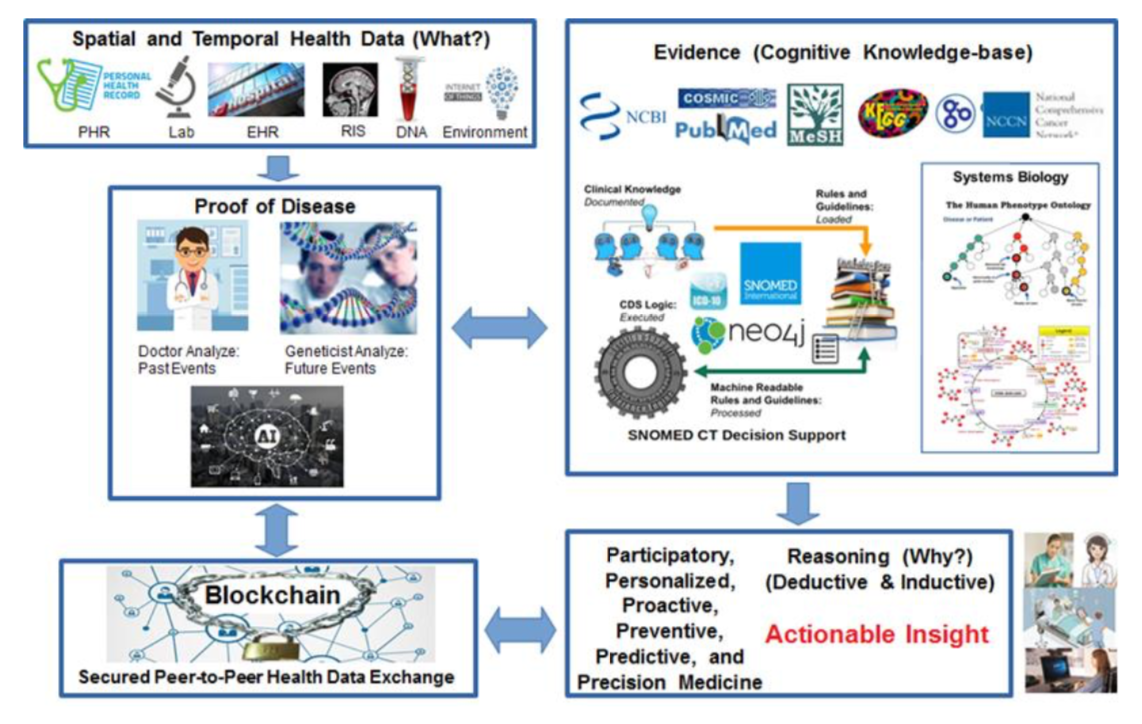
\includegraphics[width=1\textwidth]{images/example_software_architecture.png}
	\caption{Example software architecture cf.\autocite{talukder} pp.260}
	\label{example_software_architecture}
\end{figure}

In addition, there is a medical miner which validates every transaction, then translates all clinical notes into structured \ac{icd} or \ac{snowmed ct} codes. After that, all codes are stored into a smart contract. During that process, a medical expert validates whether the current onset matches any clinical pathway. 
Finally, medical experts discuss in a proper medical consensus if the data is useful for an accurate diagnosis and public health.

\section{Medical Documentation Apps}

\subsection{Overview: Smartphone apps to support self-management of hypertension}
There exist many different self-management applications for patients who suffer from hypertension. Generally, these self-management programs are likely to be effective if they track the behaviour of their users\footnote{cf.\autocite{alessa} p.1}. This means that medical self-management applications should be supported by theory-based interventions, such as identifying the target behaviour and strategies of behavioural changes needed to achieve desirable health outcomes.
\paragraph{Key functionalities}
As depicted by Alessa et al., important functionalities of medical self-management applications are stress management, communication with \ac{hcp}, self-monitoring abilities (e.g. portrayed in graphs or tables), reminders, automatic feedback and educational information.
\paragraph{\ac{bct}}
Alessa et al. describe important functionalities during the development of medical self-management applications: \ac{bct} which form a theoretical domain framework. These recommendations include:

\begin{itemize}
\setlength\itemsep{-0.5em}
  \item behaviour regulation
  \item knowledge 
  \item goals
  \item memory attention and decision process
  \item beliefs about consequences
\end{itemize}

In their study, Alessa et al. studied that many applications supporting self-management of hypertension have similar functionalities\footnote{cf.\autocite{alessa} p.2}.
Besides these findings, Alessa et al. state that privacy and security is an important issue in many health applications and that these are not available in 35\% of all applications. Moreover, it should be ensured that users are able to make fully informed decisions by equipping the applications with skills and information necessary to scrutinize the privacy and security policies. This is due to the lack of knowledge and experience of many users in privacy concerns which can be seen in the social media\footnote{cf.\autocite{alessa} p.3}.

\subsection{Blood pressure monitoring in cardiovascular medicine and therapeutics}
As mentioned above, many medical applications are developed for self-monitoring\footnote{cf. p.4ff.\autocite{white_blood_2007}}. These bring many advantages and disadvantages. On the one hand, home blood pressure measurements are representative of natural environment and can show the response to antihypertensive medication. Furthermore, it is an easy and cost-effective way for obtaining a large number of readings. 
On the other hand, the measurement monitors might be too inaccurate and only a few devices have been subjected proper validation.
White et al. mention three different monitors for home measurements: arm, wrist and finger monitors. Moreover, multiple readings, e.g. two or three per day are recommended \footnote{cf. p.23ff.\autocite{white_blood_2007}}.

\paragraph{Influence factors of hypertension}
There are multiple factors which increase blood pressure, such as age, gender, environmental factors, smoking, alcohol, medication, caffeine, stress and talking.
To be more precisely, e.g. women have lower blood pressure than men or age increases the blood pressure\footnote{cf.\autocite{white_blood_2007} pp.9}. Environmental factors describe the influence of winter or summer terms on the blood pressure values. In winter, it is possible that blood pressure values increase up to 5 mmHg. Besides, the time of date can also influence measurements. For instance, it is recommended that patients take readings in the early morning and night. And there are differences between multiple systolic measurements whereas diastolic measurements stay nearly the same. But the most important fact, stated by White et al. is that summer and exercice decrease the blood pressure measurements\footnote{cf.\autocite{white_blood_2007} pp.9}.

\paragraph{Future trends in blood pressure measurements}
As explained by White et al., it is very useful to have all readings available in an electronic form and to use these together with telemonitoring \footnote{cf.\autocite{white_blood_2007} pp.31}. In detail, the readings could be transferred automatically to the health care provider. This can help to facilitate the communication between physician and patient in an easy way so that they could form virtual hypertension clinic.

\subsection{Social web and use cases for medical apps}
As stated by Lupton et al.\footnote{cf.\autocite{lupton_apps} p.607} the current technical 'era' we are living in is the web 2.0 or social web. Social web includes sharing health and medical information with each other, e.g. patients and caregivers write about experiences and the individual health status. Often, the aim of these social webs is to control the health status by using online information and imaging.
Conforming to Lupton et al.\footnote{cf.\autocite{lupton_apps} p.608}, in healthcare projects, big data can be used to generate knowledge about healthcare, health behaviours and disease patterns. Such applications can assist in calculating diagnosis, identifying risks, facilitating health, fitness self-tracking as well as patient self-care regimes.
As reported by a study which surveyed American doctors\footnote{cf.\autocite{lupton_apps} p.610}, medication interaction apps are the first most-used and diagnosis apps the second most used category of apps.
Moreover, pregnancy apps offer greater opportunities, such as that women are engaged to real-time self-surveillance based on the produced data, such as heart rates of their embryos\footnote{cf.\autocite{lupton_apps} pp.614}. Pursuant to Lupton et al., the future potential of medical application lies in systems which enable lay people to access medical information (such as the electronic medical record) that was previously only available to healthcare practitioners or students.

In another article, Lupton et al. reported that the potential lies in automation of news or notifications which can be personalized or targeted so that doctors could contact patients directly to remind them to adhere to their tratment programs\footnote{cf.\autocite{lupton_mhealth} pp.229}.
A further example of medical applications are 'smart pillboxes' for patients suffering from diabetes\footnote{cf.\autocite{lupton_mhealth} pp.232}. 'Smart pillboxes' are wireless devices that remind patients to take their medication and alert a doctor if the patient had failed to conform to their medication regimen.
Continuing, \ac{m-health} technologies have a feedback, also called cybernetic mechanism in that they react with their users as opposed to passively provide information. To give an example, modern prosthesis or technological extensions of the body are a kind of cybernetic mechanism\footnote{cf.\autocite{lupton_mhealth} pp.234}. 
A big part of today's medical applications are surveillance systems in order to record and monitor cases of illnesses, such as obesity or infections\footnote{cf.\autocite{lupton_mhealth} pp.235}. These records might be useful to early detect epidemiological changes in the disease pattern. To give an example, 'individual medical encounters' which are conducted online enable doctors to flexibly practice personalized surveillance over each of their patients. At this point, another term occurs: 'surveillance knowledge' which refers to the digital data produced in the surveillance and can be useful for the individuate users.

\paragraph{Blockchain solution for accurate medical decisions}
As stated by Talukder et al. a significant amount of today's diagnosis in \ac{ncd} is 	
erroneous or unwanted\footnote{cf.\autocite{talukder} p.263}. The term \ac{ncd} implicates disease caused by an unheallthy lifestyle, the proper environment or genomic causes over a long time and come up with confusing signs and symptoms.
Talukder et al. mention 'P6'-Medicine which describes medicine using six adjectives starting with the letter 'p': medicine needs to be participatory, personalized, proactive, preventive, predictive, precision medicine.
As a requirement list for health data, Talukder et al. describe important features as follows: 

\begin{itemize}
\setlength\itemsep{-0.5em}
  \item secured (the anonymity, privacy, confidentiality of health data must be approved)
  \item systems which provide health data must have a zero down-time 
  \item the integrity of the health data must be ensured
  \item the systems must be ubiquitous which implies an unlimited availability
  \item machine understandable (all health data should be conform to international standards and should be able to be distributed over multiple systems)
  \item health systems should be resistant against fraudulent hacking
\end{itemize}

\section{Chatbots} 

\subsection{Use cases of chatbots}
The main advantage of chatbots is to provide a 24-hour customer service with personalized interaction and no waiting time\footnote{cf.\autocite{akhtar} pp.297}. 
Besides, the data retrieval from conversations with chatbots provides many possibilities. To be more precise,  modelling, profiling, analyzing and understanding users becomes increasingly important in many different indrustries and count as key to success in todays data driven world. 
Akhtar et al. analyzed chat conversations between customers and the chatbot of a telecommunication company in order to find out the user's topics of interest and how to satisfy users. As described by Akhtar et al., the tests of the chatbot were splitted into different activities, such as text mining techniques (feedback comments), event sequence analysis, frequent term extraction, analysis of bigrams/trigrams. 
During data preprocessing, Akthar et al. used the following methods:
\begin{itemize}
\setlength\itemsep{-0.5em}
  \item[1.] corpus generation
  \item[2.] eliminating extra white space
  \item[3.] stopwords removal
  \item[4.] tokenizing
  \item[5.] stemming
  \item[6.] creating term-document matrices
\end{itemize}

The main challenges during the data analysis process are data availability, the access to further user information (e.g. contract details or age in order to generate an user model) and the distinction between different user types and different personality structures.

\paragraph{Types of dialog systems}
In general, dialog systems can be divided into two kinds of systems. On the one hand, there are task-oriented systems which are appropriate for short conversations and built for a certain purpose. On the other hand, there are non-task-oriented systems which are built for longer and more complex interactions with the purpose of imitating human conversations\footnote{cf.\autocite{akhtar} pp.399}.

\subsection{A deep learning question-answering specialized chatbot for medical students}
During their studies, medical students have to take an exam which is called \ac{osce} where they interact with a 'standardized' patient played by an actor who simulates the symptoms and intents of the patient\footnote{cf.\autocite{zini} p.2}. The aim of this exam is to test and assess the students' abilities and social interaction and diagnosis skills.
Since in practice, there are not many actors who can play a patient's role, Zini et al. developed a virtual patient and chatbot system which works with \ac{nlp} techniques.

Figure \ref{vp_architecture} shows the architecture of the developed system to create a virtual patient. Zini et al. used a \ac{cnn} and \ac{lstm} network in order to learn domain specific word embeddings, sentence embedding and answer selection models.
The embeddings model which is outlined by a red rectangle in figure \ref{vp_architecture} is trained on a corpus of medical documents.
In Figure \ref{vp_architecture}, there is a \ac{nlp} engine outlined by a red rectangle. By using a supervised learning scheme to learn a mapping between question and answering pairs and judgement of correct match, this \ac{nlp} engine should correctly answer questions based on a script.

\begin{figure}[h!]
	\centering
	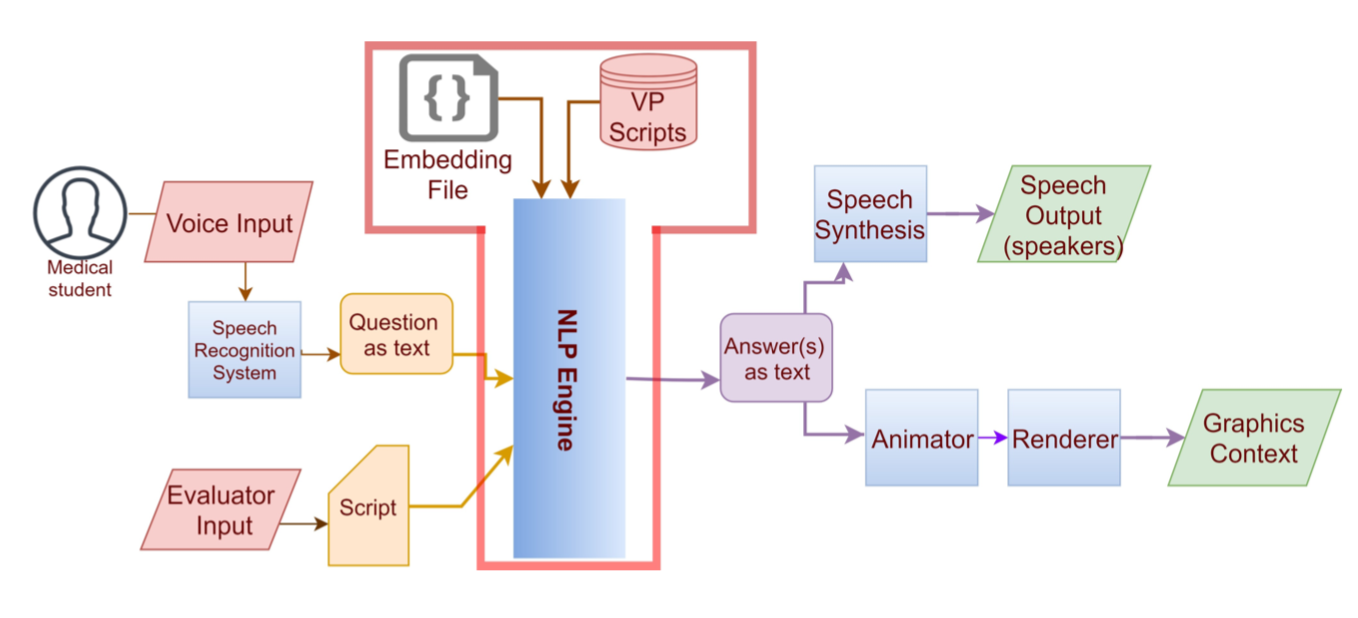
\includegraphics[width=1\textwidth]{images/vp_architecture.png}
	\caption{Virtual patient software architecture cf.\autocite{zini} p.3}
	\label{vp_architecture}
\end{figure}

The aim of the developed system was to create a deep learning framework for answer selection in the medical domain and to create domain-specific word and sentence embedding models. Additionally, a question and answering corpus should be created for \ac{osce}s.

\paragraph{Question and Answering systems}
According to Zini et al. there are two types of question and answering systems\footnote{cf.\autocite{zini} pp.4}. First of all, there is open domain question and answering which uses very specific terminology. Secondly there are restricted domain question and answering systems which are broader in their scope. These are for example insurance-related deep learning question and answering systems which make use of two baseline models: \ac{bow} and \ac{ir} model. 

\subparagraph{Question Answering Paradigms}
There are several types of conversations which can be designed by building a chatbot\footnote{cf.\autocite{akhtar} p.398}. Generally, there can be distinguished between two different paradigms: information-retrieval based Question and Answering and knowledge-based Question and Answering. The first type describes the mechanism to define short texts as answers to a user's intent. On the opposite, the second type describes how to in natural language. The answers are stored into a full-related database and the conversation works simply with a rule-based method.

\chapter{Analysis and Development}

\section{Experimental set-up} \label{first_ideas}

First of all, the developed chatbot includes information about blood pressure and was built to remind patients of their measurements. Secondly, based on the measured data, analysis can be done in order to react earlier to outliers. Thirdly, a generated report is sent to the doctor via email so that he can get more insights about the blood pressure values of his patients and can improve the treatment.
One of the main challenges during development was the process of providing information about the disease to the patient. Is it possible to include information about different types of blood pressure into the automated conversation with a chatbot? Or does it overwhelm the conversation's use case? Is it useful to let the user ask questions like: 'What are the different types of hypertension? Am i a high-risk patient?' 
Or should these information be provided as a video or a simple web page with long articles to read? Might the patient or user be aborred after a while of talking to a chatbot who only knows answering his questions in the same way?
Of course, a chatbot can be developed in a more intelligent way to never provide the same answer and to answer more precisely to a users' intent. But this requires a lot of training and testing. 
For that reason, in the first version of this chatbot, four intents and dialogs have been designed and implemented with the focus of the instructions to measure correctly and regularly. 
In a second or third version, it is possible to focus more on the improvement of providing information about the disease (by not doing this in the style of question and answering).

\section{Software architecture}

Figure \ref{architecture_0102} gives an overview of all developed components. Quite above, there is the Watson Assistant instance, running in the IBM Cloud. Beneath Watson Assistant, a NodeJS server opens the session and sends messages from the client to the Assistant and backwards. The NodeJS server connects the cloud and the frontend by implementing \ac{http} requests and responses. Finally, there is the AngularJS application running locally and creating a \ac{json} reporting file every few minutes. This reporting file includes all messages, with the user from whom it was send and a timestamp. It can be used to analyze the data and to create profiles of the patients.

\begin{figure}[h!]
	\centering
	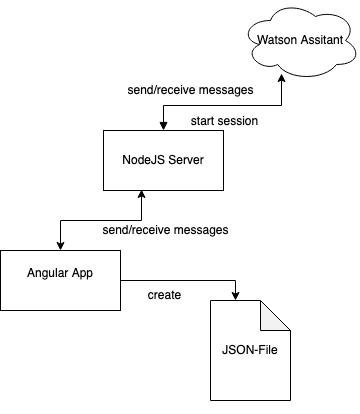
\includegraphics[width=0.7\textwidth]{images/architecture_0102.png}
	\caption{Architecture diagram of developed system}
	\label{architecture_0102}
\end{figure}

\section{Setup of Angular Frontend} \label{frontend}
In order to provide a comfortable way to chat and view all retrieved and measured data, an angular application was built and run locally (see figures \ref{angular_01} and \ref{angular_02}). Three open source libraries, such as Nebular\footnote{cf.\autocite{nebular}}, Apache Echarts\footnote{cf.\autocite{echarts}} and Openlayers Maps\footnote{cf.\autocite{openlayers}} were included to the application (see figures \ref{angular_01} and \ref{angular_02}). Nebular is a Javascript library that has certain themes (e.g. light, dark etc.) and a many components, such as a chat UI (which allows to send messages and different file types such as documents or images or videos). It also allows to send a location by defining longitude and latitude parameters. Generally, building up an Angular webpage (see also figure \ref{angular_01}) is a very state-of-the-art solution and enables the development of mobile applications and the usage of diverse libraries.

\begin{figure}[h!]
	\centering
	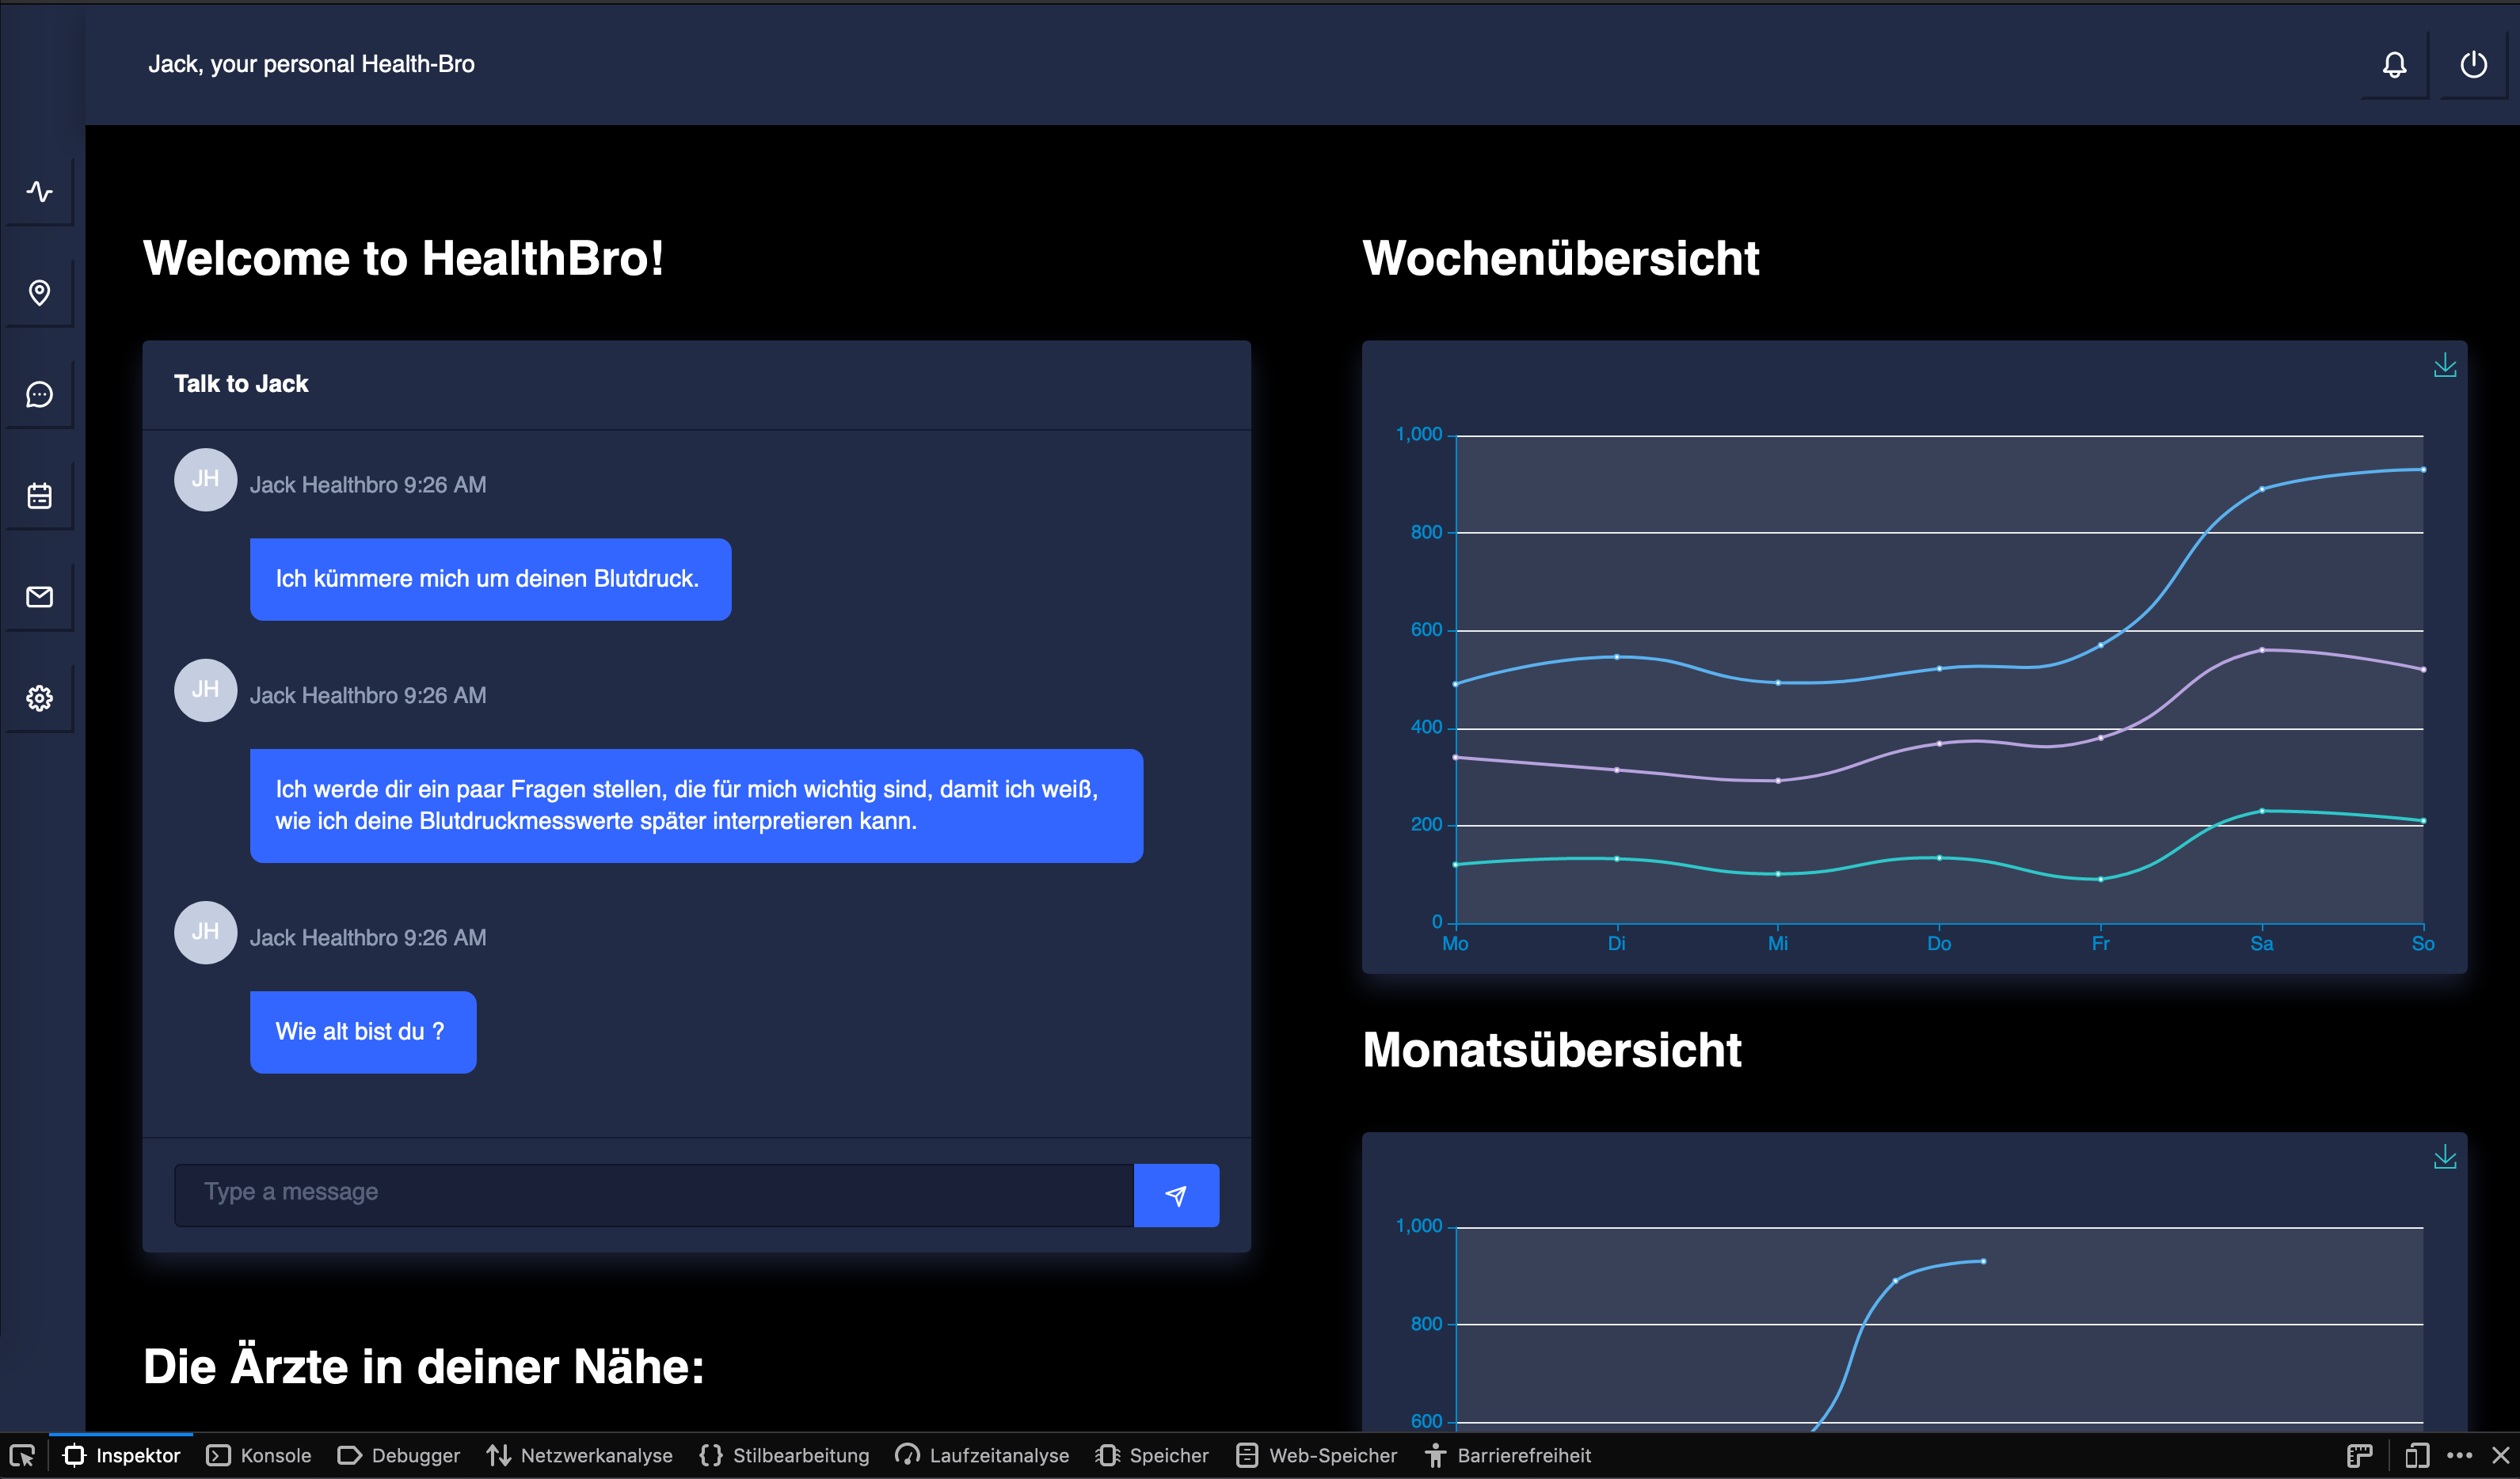
\includegraphics[width=1\textwidth]{images/angular_01.png}
	\caption{Angular Frontend (top page), chat UI and diagrams of measured values}
	\label{angular_01}
\end{figure}
\begin{figure}[h!]
	\centering
	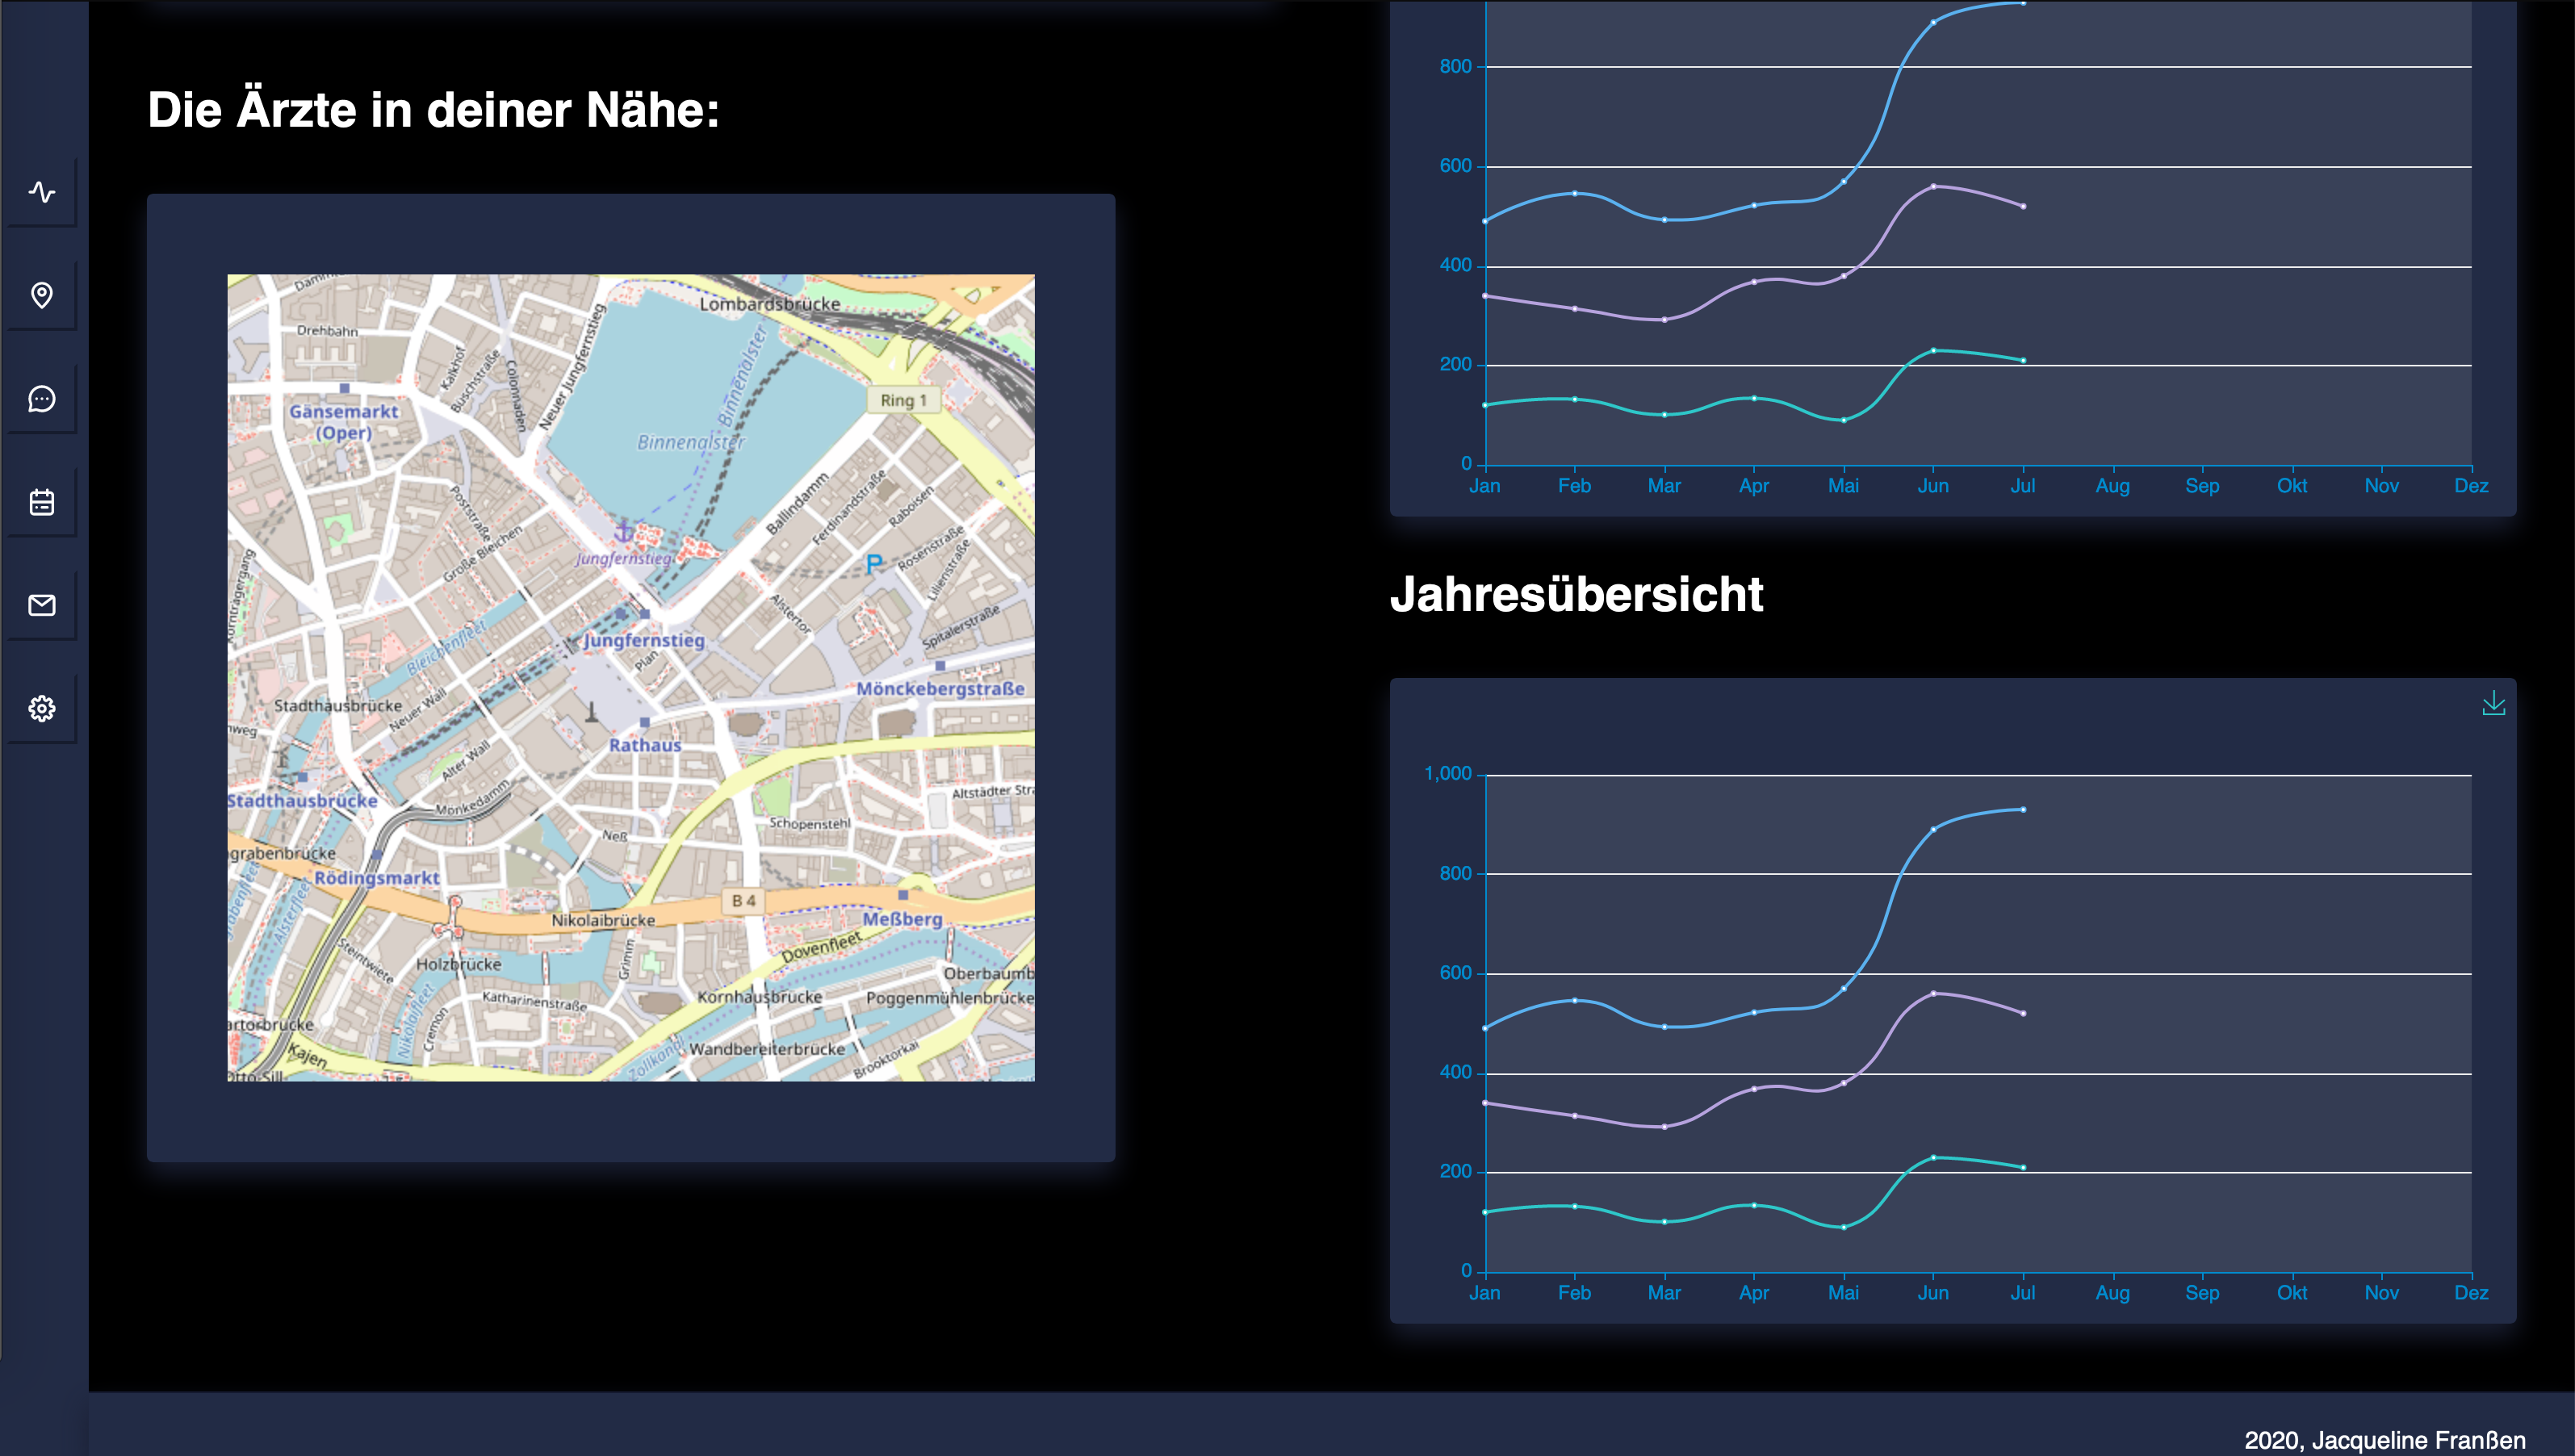
\includegraphics[width=1\textwidth]{images/angular_02.png}
	\caption{Angular Frontend (bottom page), map to show the nearest doctors}
	\label{angular_02}
\end{figure}

Secondly, Apache Echarts is also a Javascript library which offers a huge variety of diagrams and maps, such as bar, line, pie and other special diagrams (including different animation modes, overlays and tooltips). At the beginning, the line chart was used to display the weekly, monthly and yearly overview of measured pulse, systolic and diastolic values. For future use cases, it can be also useful to display other charts of Echarts or tables to better understand trends.
The third Javascript library that was used, is called Openlayers Maps and is an open source software. It is widespread and many projects rather use Openlayers \ac{api} than Google Places \ac{api} because their \ac{api} calls are very expensive. Openlayers Maps has many different modes and overlays. Besides, certain places can be marked by different icons.
All in all, the three described libraries are very well documented and are easy and ready to use after installation, so that the focus could be spent more on developing the Watson Assistant dialog described in the next paragraph.

\section{Development of Watson Assistant Dialog}

\subsection{Intent model} \label{intentmodel}
The chatbot was built according to the information given by the webpage of "Deutsche Hochdruckliga", a german organization for patients who suffer from hypertonia\footnote{cf.\autocite{hochdruckliga}}. 
To better understand the users and patients an intent model with four intents was developed. 
The four intents are described by table \ref{table}. 

\begin{table}[h!]
	
		\begin{tabular}{ |l|l| } 
				\hline
				Intent & User input  \\
				\hline

				%\multirow{4}{4em} \\
				Definition of hypertonia  & What is hypertonia?  \\ 
				Curses of hypertonia & What are the implications or curses of hypertonia? \\ 
				Blood pressure measurement &  I am measuring my blood pressure.\\ 
				Measurement tutorial & How should i measure my blood pressure? \\ 
				\hline
		\end{tabular}

      \caption{Developed intents and specification} \label{table}         
\end{table}

These four intents were used to define and develop four typical dialogs, displayed in figure \ref{dialog_diagram_01}, \ref{dialog_diagram_02}, \ref{dialog_diagram_03} and \ref{dialog_diagram_04}.

\begin{figure}[h!]
	\centering
	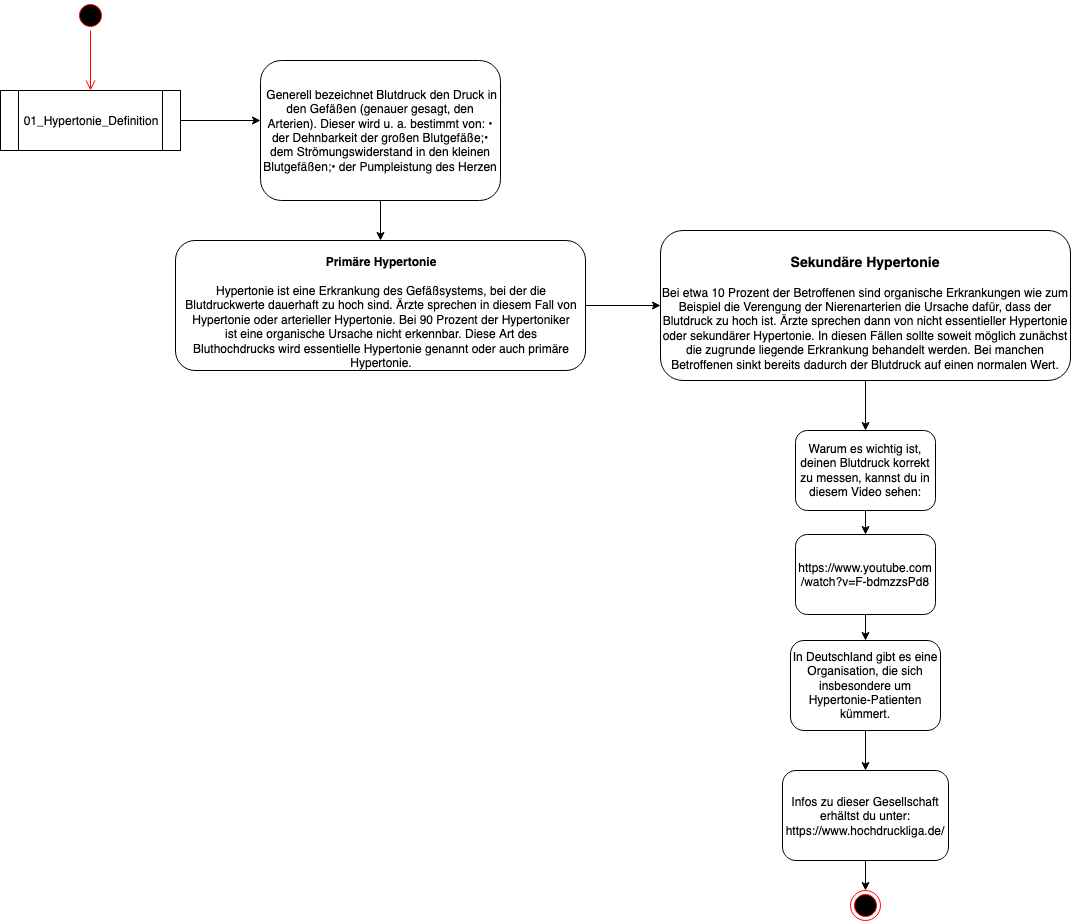
\includegraphics[width=1\textwidth]{images/01_Hypertonie_Definition.png}
	\caption{Dialog diagram: definition of hypertonia}
	\label{dialog_diagram_01}
\end{figure}

\begin{figure}[h!]
	\centering
	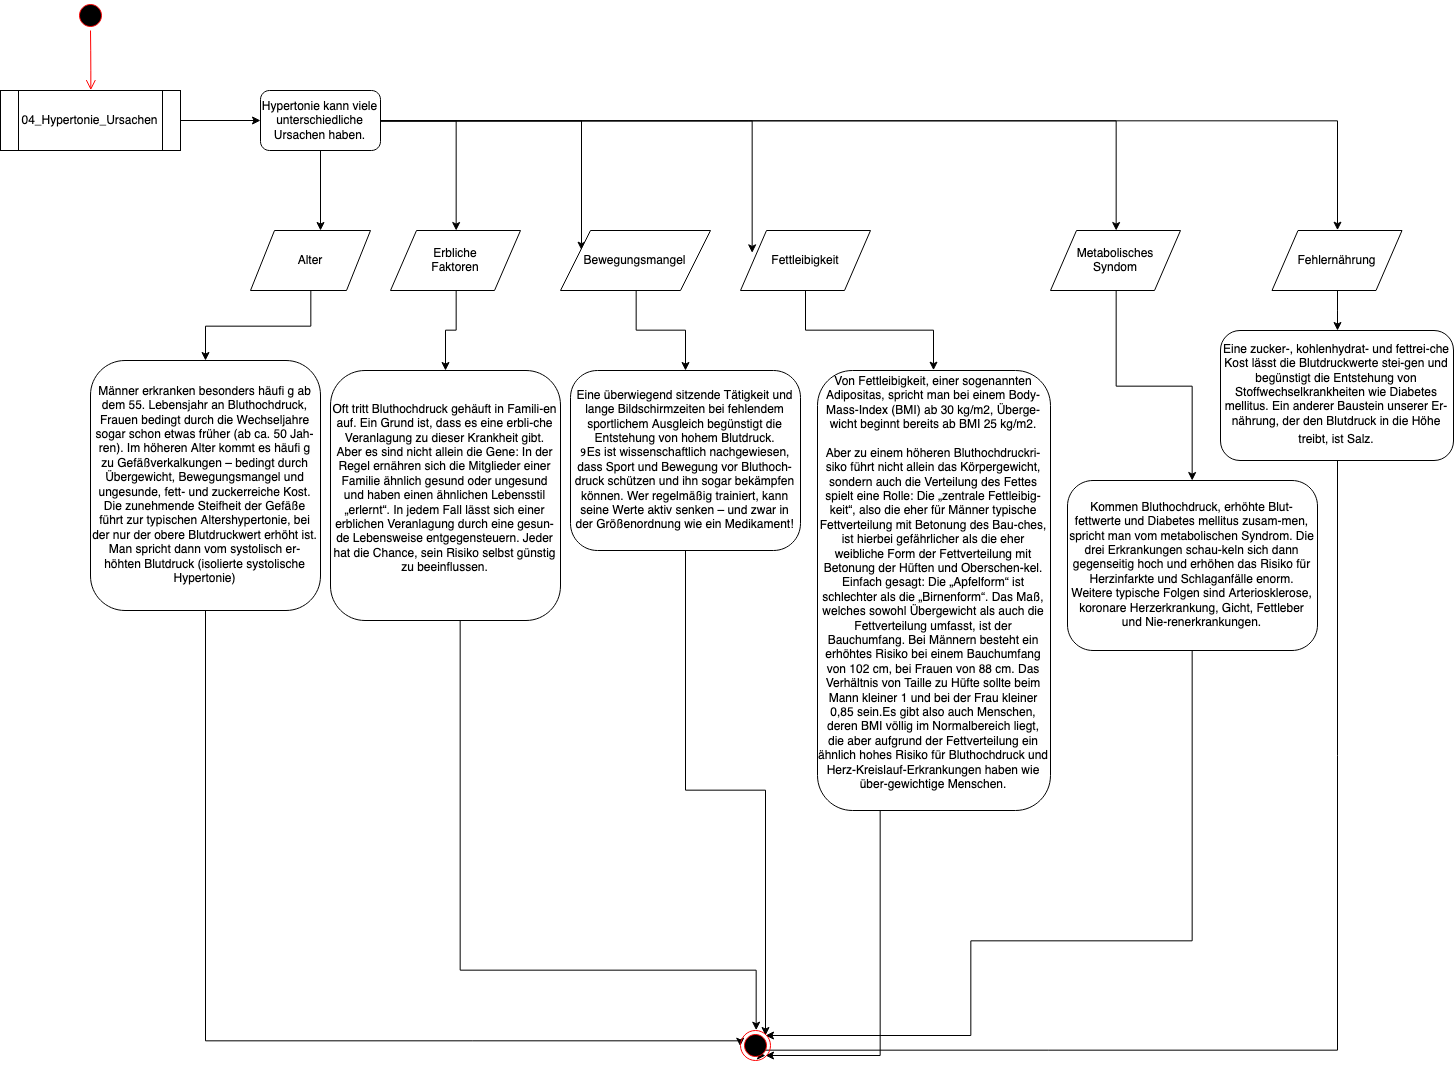
\includegraphics[width=1\textwidth]{images/02_Hypertonie_Ursachen.png}
	\caption{Dialog diagram: curses of hypertonia}
	\label{dialog_diagram_02}
\end{figure}

\begin{figure}[h!]
	\centering
	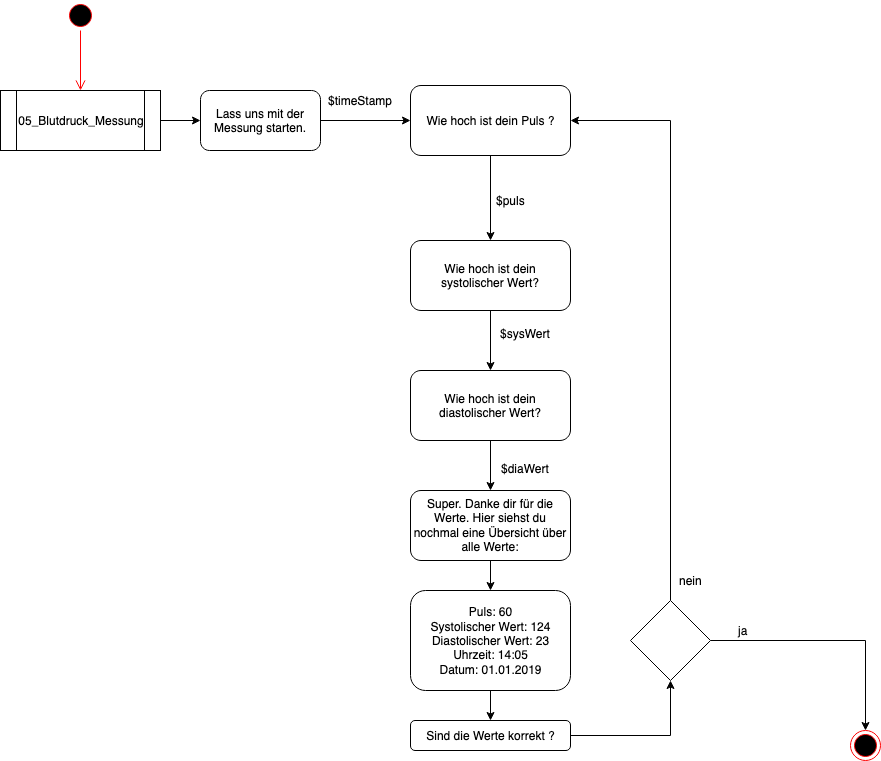
\includegraphics[width=1\textwidth]{images/03_blutdruck_messung.png}
	\caption{Dialog diagram: blood pressure measurement}
	\label{dialog_diagram_03}
\end{figure}

\begin{figure}[h!]
	\centering
	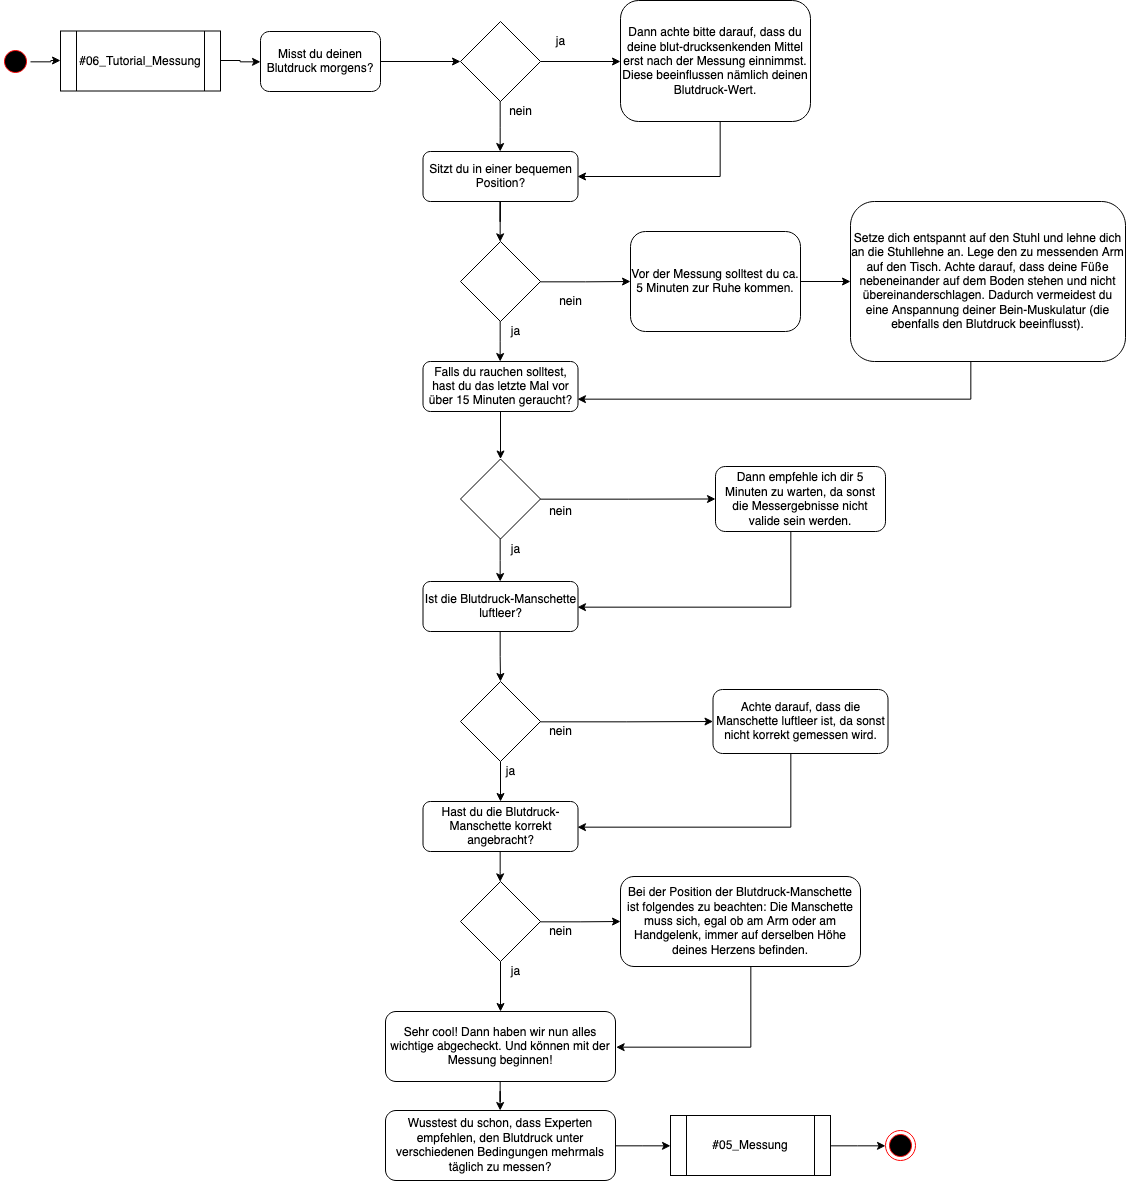
\includegraphics[width=1\textwidth]{images/06_tutorial_messung.png}
	\caption{Dialog diagram: measurement tutorial}
	\label{dialog_diagram_04}
\end{figure}

\subsection{Watson Assistant implementation}
In the following, the implemented dialog including all entities and intents are described. They have been developed according to the Watson Assistant documentation \footnote{cf.\autocite{wa_docu}}.
Basically, 16 entities (see figure \ref{wa_entities}) and 17 intents (see figure \ref{wa_intents}) were defined. Entities give examples of an user's input whereas intents describe the 'wish' or what the user wants to know.
\begin{figure}[h!]
	\centering
	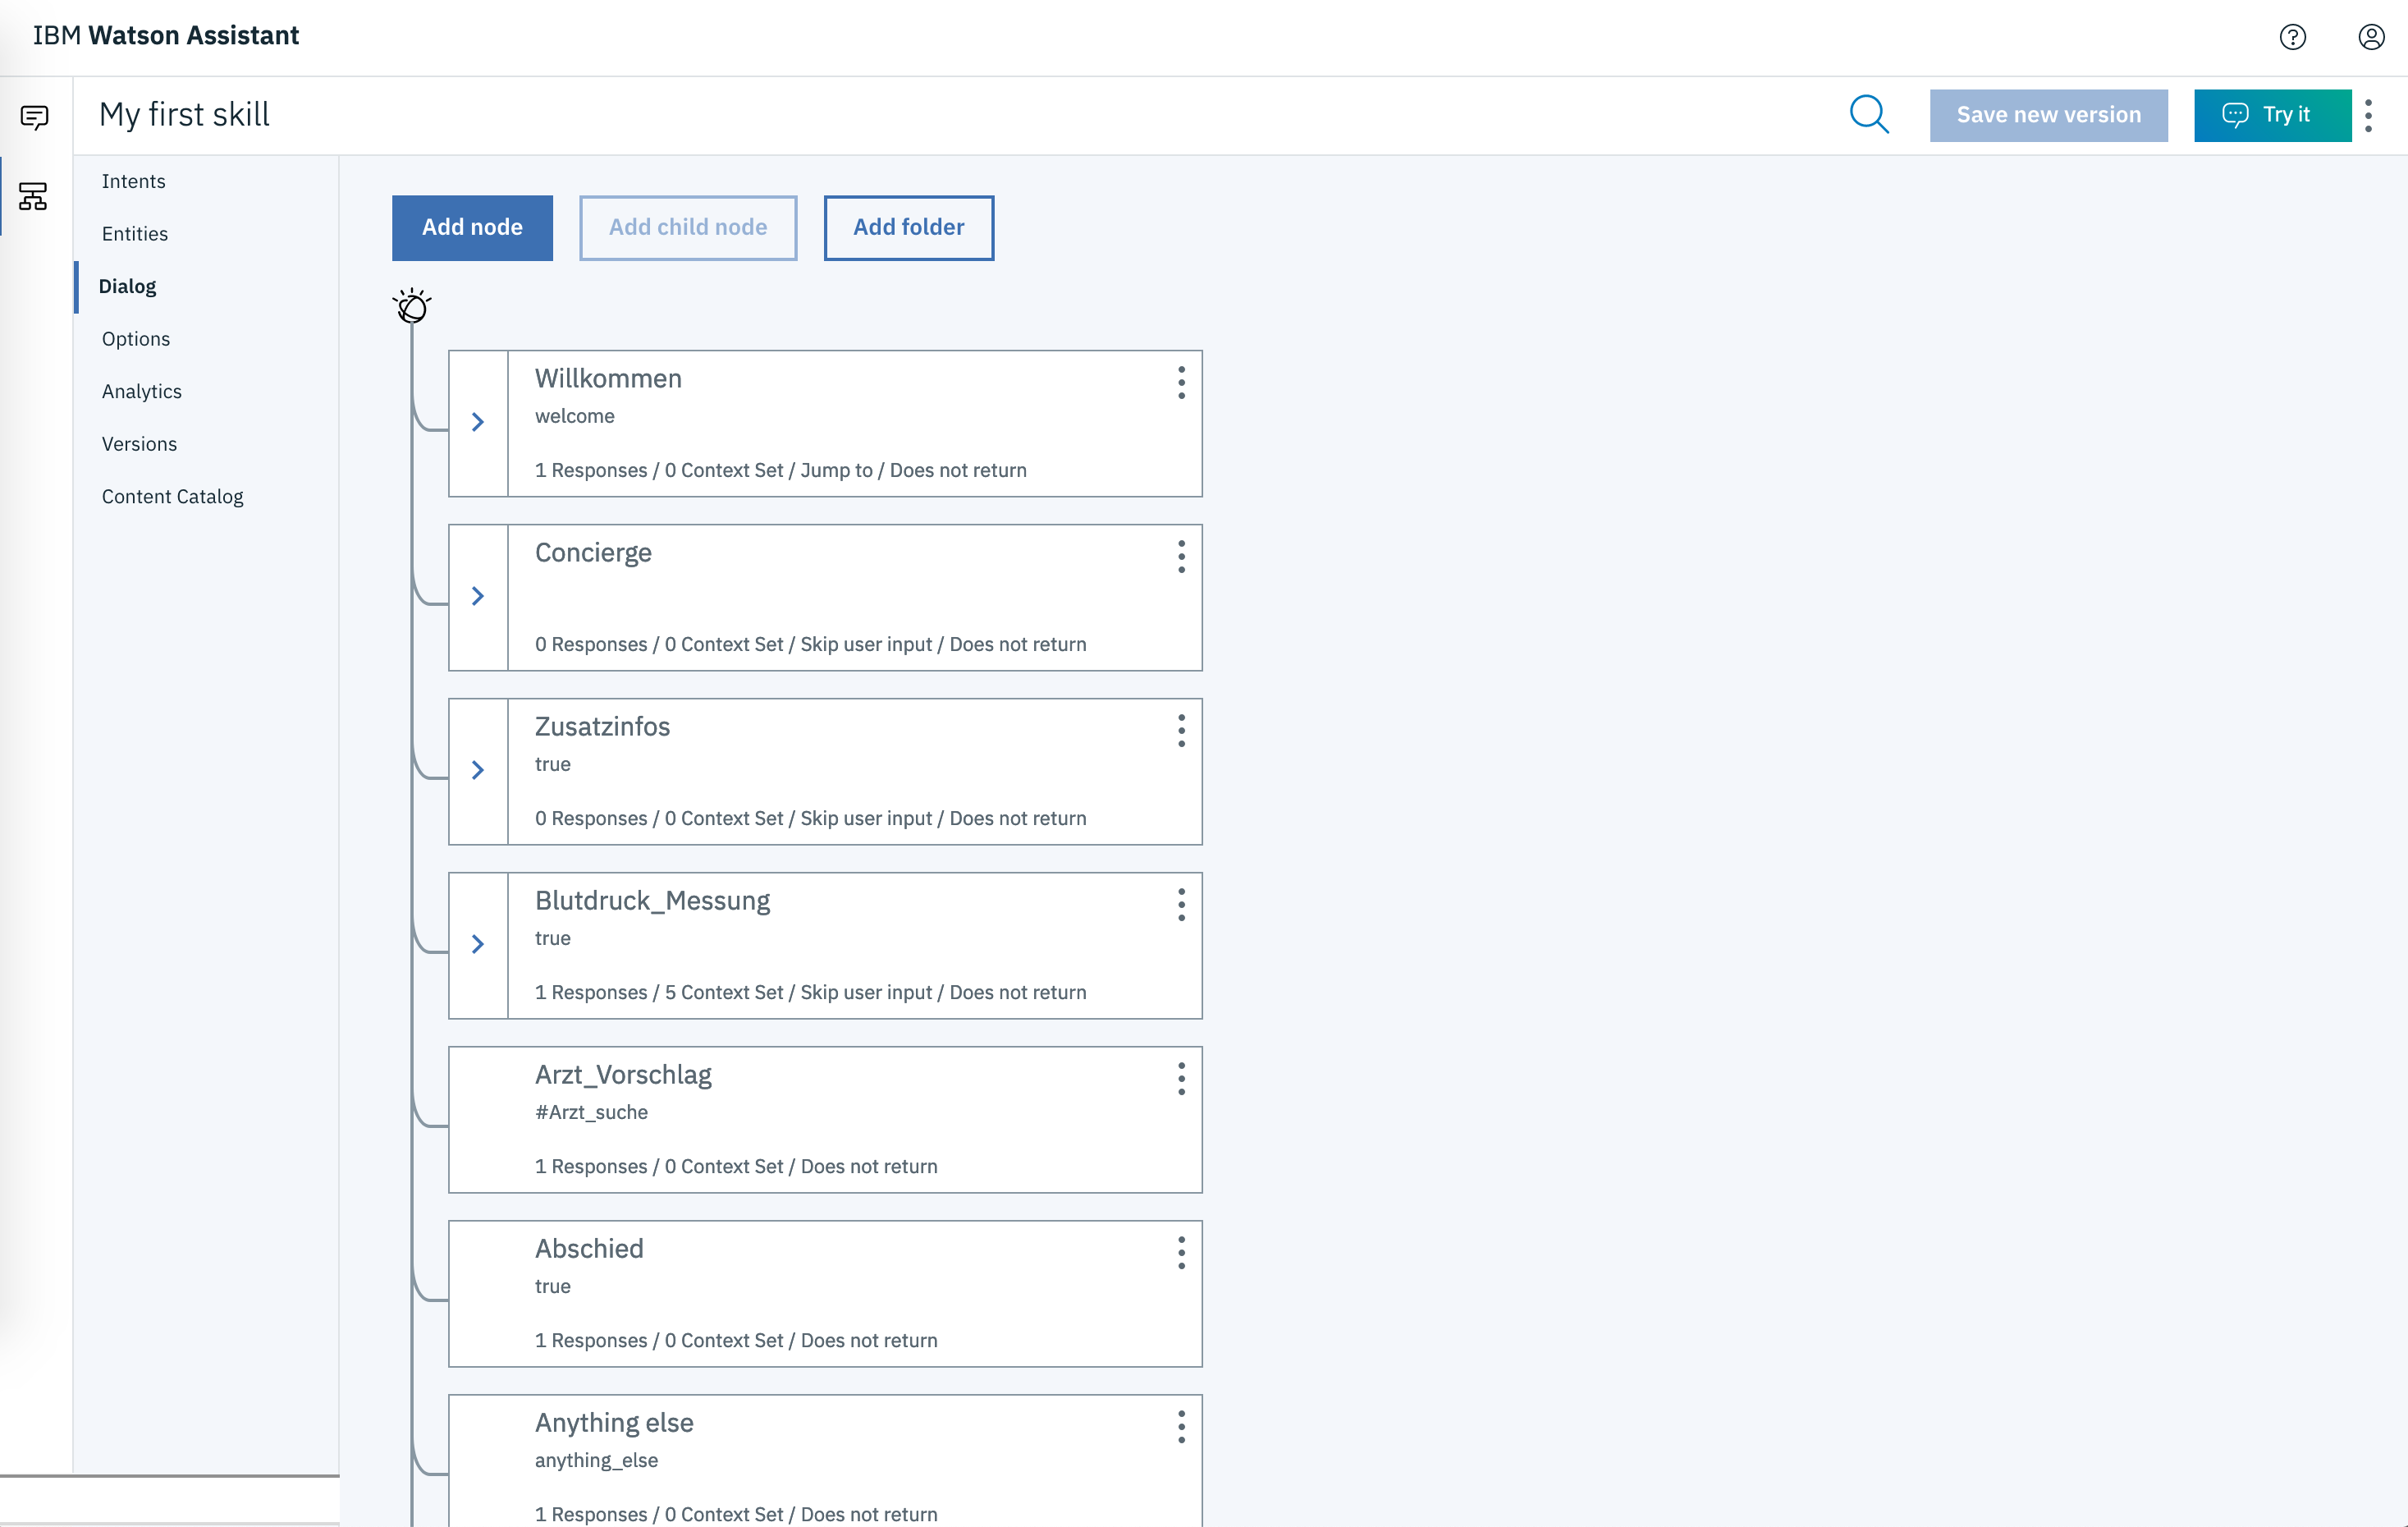
\includegraphics[width=1\textwidth]{images/WA_dialog.png}
	\caption{Watson Assistant dialog}
	\label{wa_dialog}
\end{figure}

\begin{figure}[h!]
	\centering
	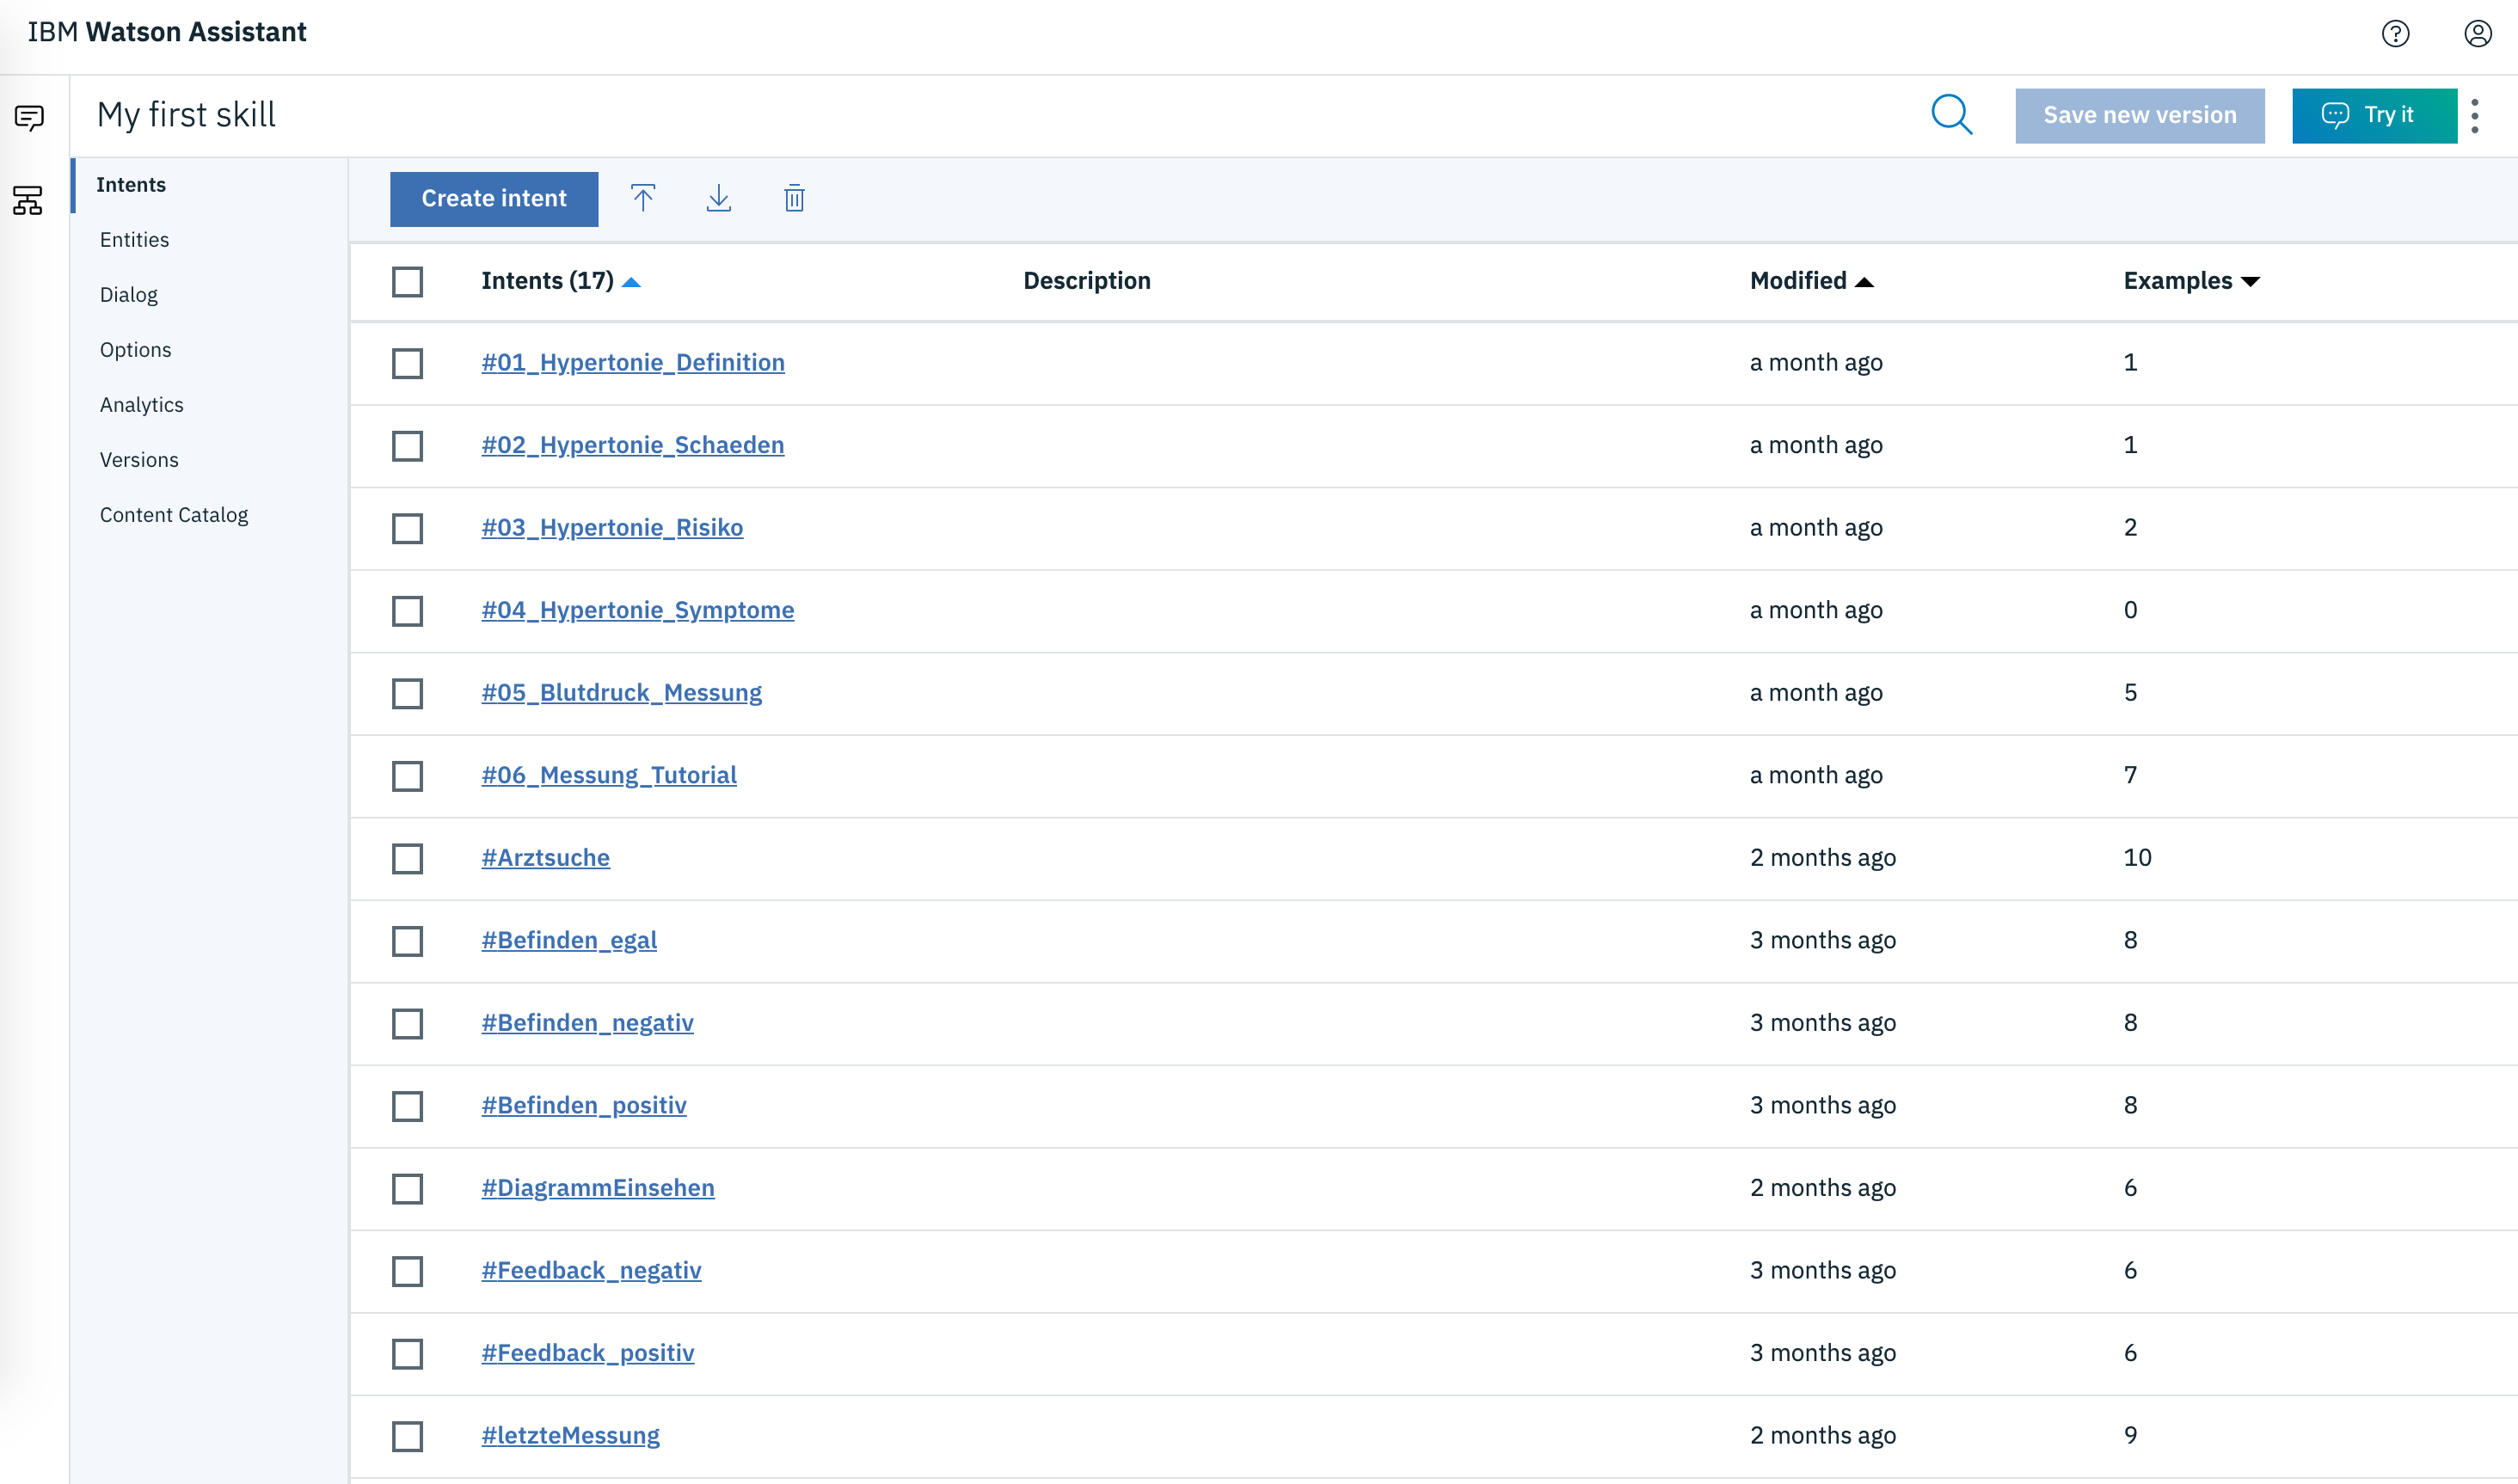
\includegraphics[width=1\textwidth]{images/WA_intents.png}
	\caption{Watson Assistant intents}
	\label{wa_intents}
\end{figure}

\begin{figure}[h!]
	\centering
	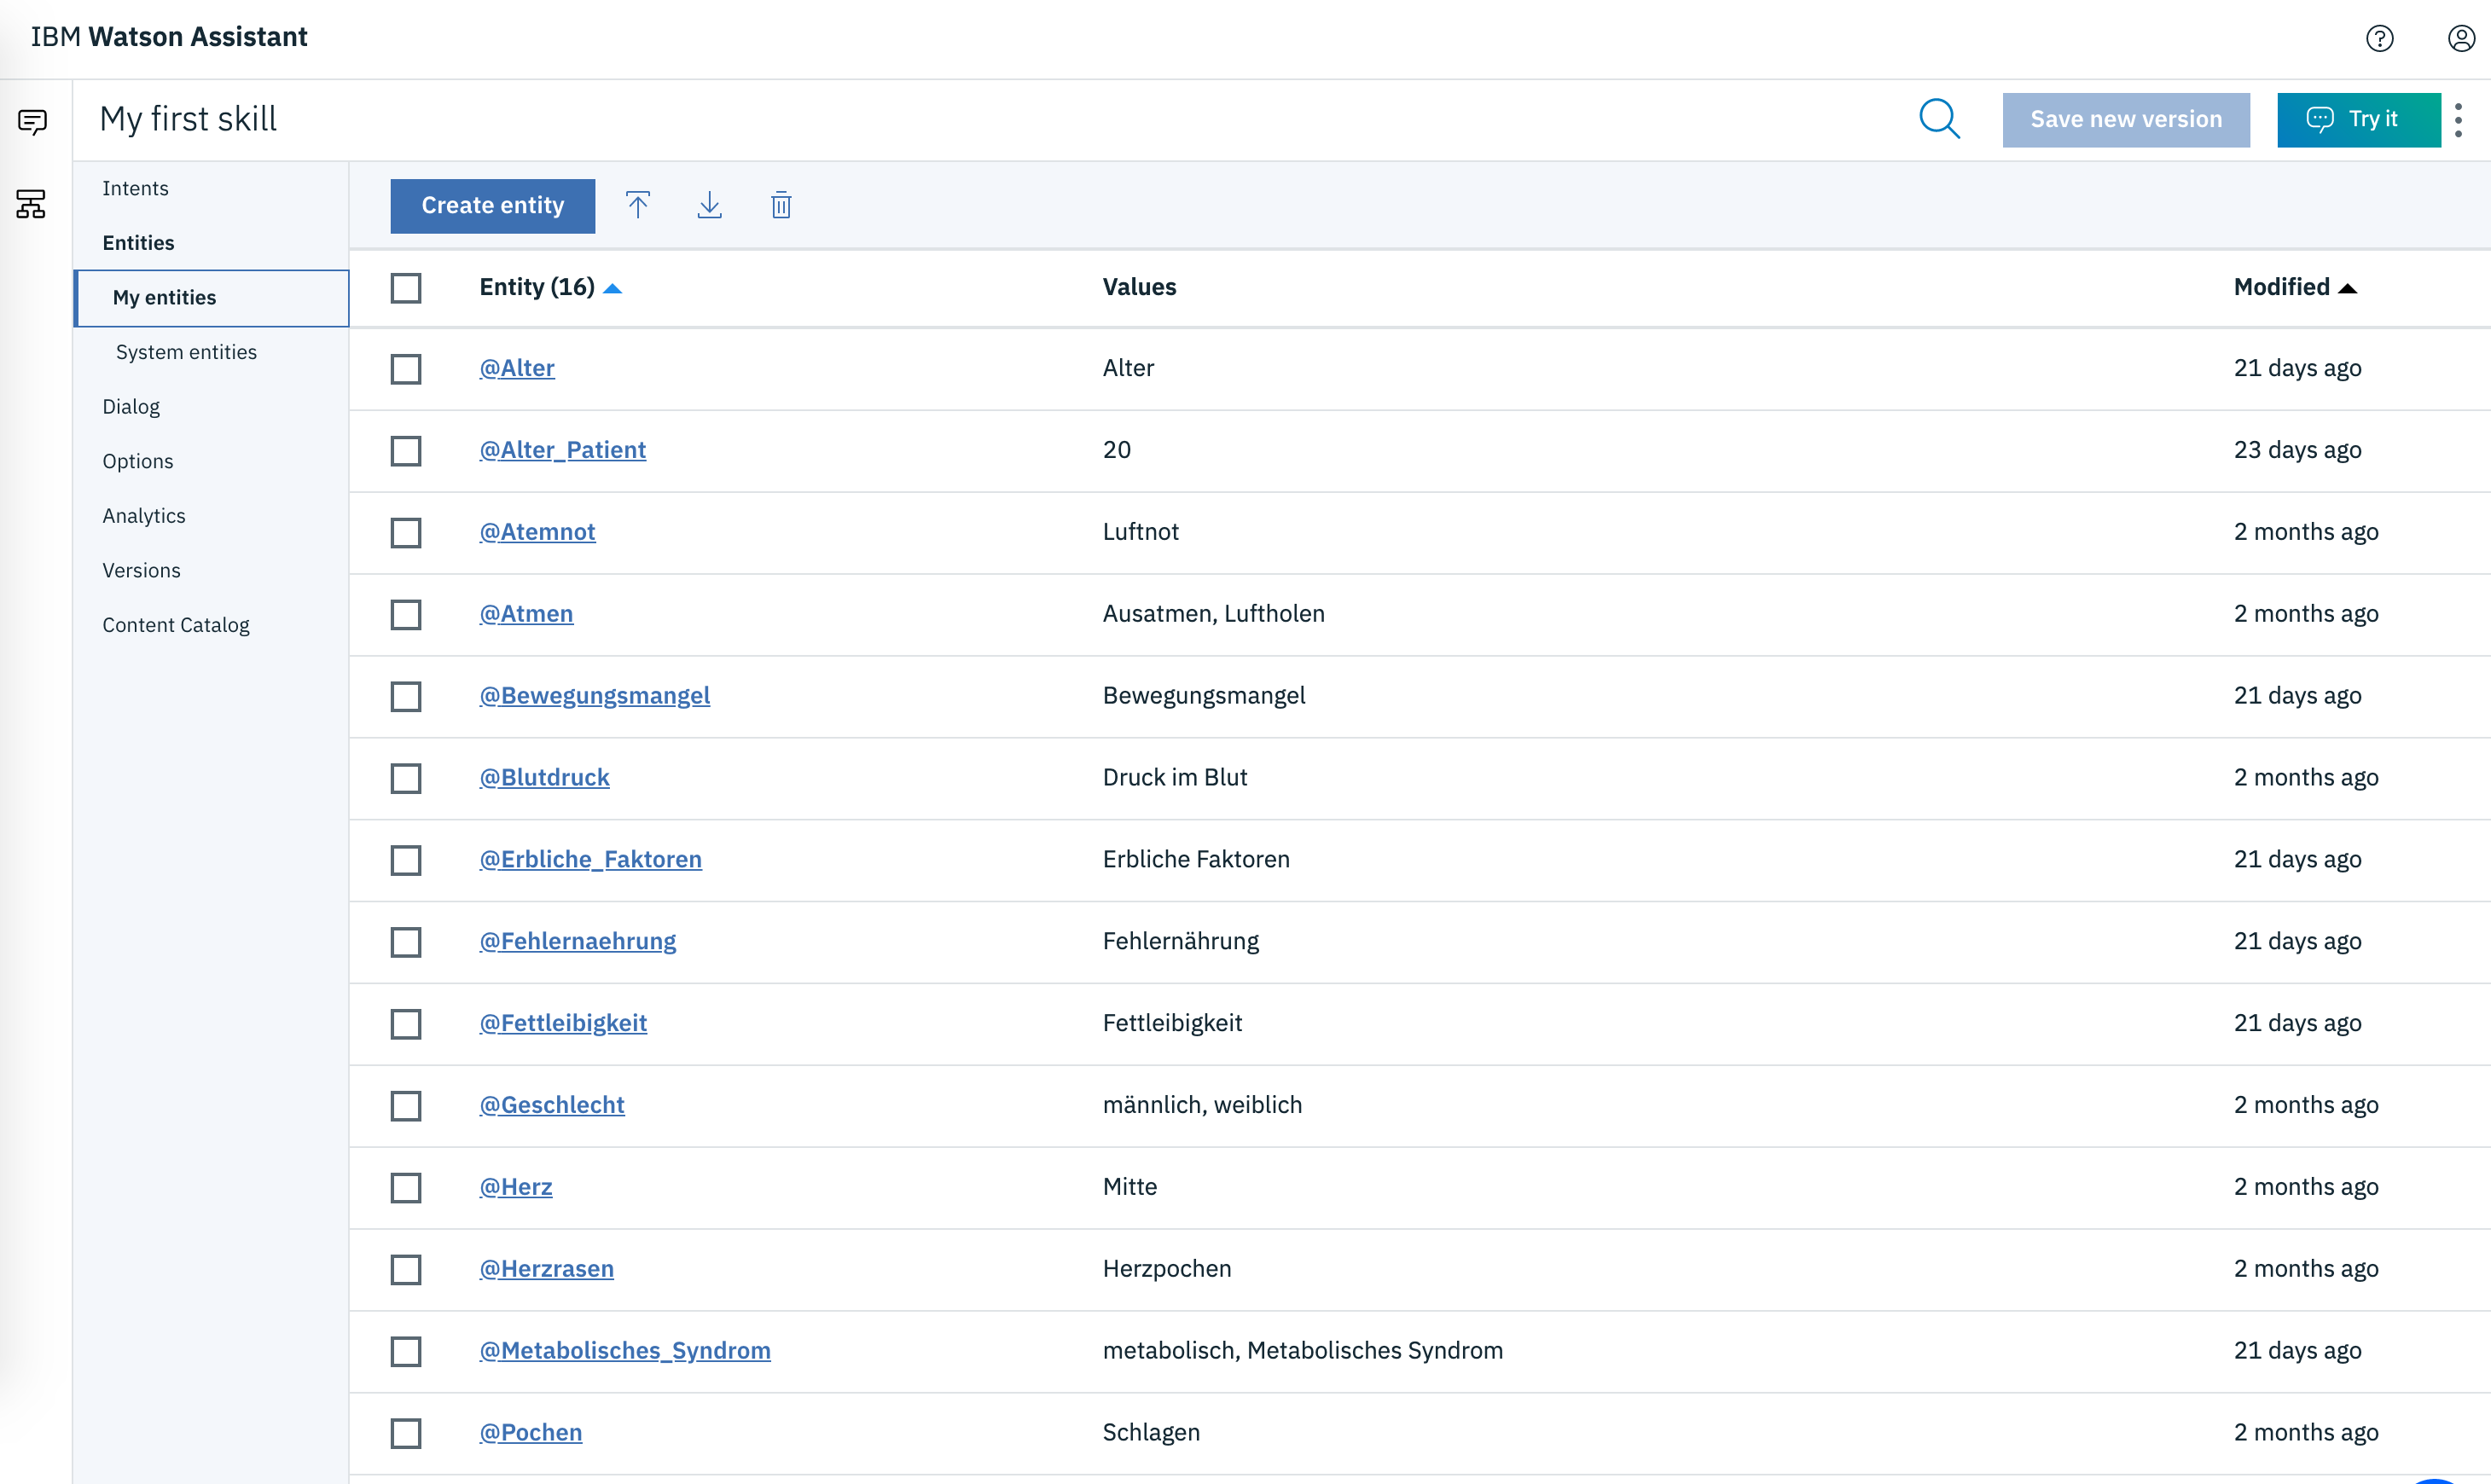
\includegraphics[width=1\textwidth]{images/WA_entities.png}
	\caption{Watson Assistant entitities}
	\label{wa_entities}
\end{figure}
The dialog (see figure \ref{wa_dialog}) includes 

\begin{itemize}
\setlength\itemsep{-0.5em}
  \item a welcome node
  \item a concierge node which asks the general data (e.g. age, gender, height, weight etc.) and starts the tutorial
  \item an additional information node (if the user wants to know more about hypertonia)
  \item a measurement node
  \item a recommendation of doctors node.
\end{itemize}

The conversations are implemented as explained in section \ref{intentmodel}. In Watson Assistant, each node can be defined with a condition. If the value of the condition is true, the response of the node is returned to the user. If it is false, the next node (usually above the other node) is checked for its condition. In case of no appropriate node, there should be defined a 'anything-else' node which always return a response if the other nodes were not true. Generally, the response of the anything else node is something like 'Sorry, i did not understand. Could you try to rephrase your question, please?'.
When it comes to the four intents, the first implementation included passing all nodes, one after another. But as mentioned in section \ref{first_ideas}, there are some special nodes which should be passed only once per user whereas other should be displayed regular intervals. This was not implemented in the component Watson Assistant (even though there are possibilities, such as defining 'slots' for certain \ac{ir} routines) but in the frontend component (Angular web application) which is explained in section \ref{frontend}. 

\section{Connect Watson Assistant and Angular frontend}

To be able to connect to the Watson Assistant instance on IBM cloud, the \ac{api} Version 2.0 had to be called. First of all, the current sessionId was requested to be able to interact with Watson Assistant. After that, a get request was executed to let the chatbot start the conversation. Everytime, the user sends a message to Watson Assistant, a post request is sent to the \ac{api}. The response is the answer of the current node in Watson Assistant\footnote{cf.\autocite{wa_api_v2}}. In order to define the conversation's direction, the intent's probability is calculated (every intent has its own learning set which at least should include six sentences). If the algorithm detects one of the given learning sets of an intent, its answer is displayed by the chat \ac{ui}

\subsection{Development of email service to send reports every two weeks to the doctor}

Another challenge was the way to automatically ask the user for his measured data. Most chatbot only helps in certain situations including precise user intents, e.g. the question 'When should i measure my blood pressure?'. By implementing a python script for data analysis an alarm was created to remind users every five hours or once a day.
In order to face this problem or use case, a routine for sending an email including a timer was implemented. Regarding the future, the routine of sending an email should be migrated into the frontend or the doctor's system so that he will be informed as soon as possible. 

\section{Predictive Analytics: Creating a model to predict cardiovascular disease} \label{predict}
Generally, it is hard to let an algorithm diagnose cardiovascular disease if only looking at the dataset above. In practice, it needs the experience of a doctor and many different measured values in different situations (e.g. in stress situations or in relaxing situations). Nevertheless, for analytics it is very interesting to test if for example a neural network could learn on the given dataset and could predict the probability of a cardiovascular disease for a given patient. 

\subsection{Dataset}
Since this scientific article focusses on the development and setup of Watson Assistant API and the Angular Frontend, real user data was not used for evaluation and analysis. Instead, a given Kaggle dataset\footnote{cf.\autocite{kaggle}} was used for calculating the diagrams. It contains 70000 entries of different patients and 12 characteristics. These 12 characteristics describe:
\begin{itemize}
\setlength\itemsep{-0.5em}
  \item age (in days)
  \item gender
  \item height
  \item weight
  \item systolic value
  \item diastolic value
  \item cholesterol (1: normal, 2: above normal, 3: well above normal)
  \item gluc (1: normal, 2: above normal, 3: well above normal)
  \item smoke (binary)
  \item alco (binary, consume of acohol)
  \item active (binary, physical activity)
  \item presence or absence of cardiovascular disease (binary) 
\end{itemize}  

The first four characteristics (age, gender, height, weight) are objective features and give factual information. After that, systolic, diastolic, cholesterol and glucose values are examination features and include the results of medical examination. The last four features (smoke, alcohol, active and the presence of cardiovascular disease) are subjective information and given by the patient.

\subsection{Development of neural network} \label{python}
Based on the given Kaggle Dataset, a neural network using Keras library\footnote{cf.\autocite{keras}} was developed. This script builds up a neural network for an intelligent and fast way to find out whether a person with given health characteristics has a higher or lower risk to suffer from cardiovascular disease. Therefore, all given features were important for the analysis and none was eliminated. Moreover, the \ac{bmi} was added and calculated by the given height and weight values. 

During the first step of analysis, the dataset had to be cleaned from null values. After that, a correlation matrix was built up and calculated to check whether all features are relevant for the analysis. This was implemented by using seaborn's (a python library for diagrams\footnote{cf.\autocite{seaborn}}) function 'heatmap'. The produced heatmap (see appendix \ref{appendix b}) shows the parameters of the dataset and how they correlated with the classification variable 'cardio' (which means that the person suffers from cardiovascular disease or not). The result of the correlation matrix shows that all features are relevant for the analysis.

After that, a model with 10 input variables and one target variable was created. The dataset was splitted into both a training and a test set. 30\% of the dataset was declared as test set and the target variable was removed. 
The neural network was built up with three layers: two hidden and one output layer. The first two hidden layer contain 5 nodes each of them (since there are 10 input variables) and are activated by a simple 'relu' activation function. The third layer, the output layer was built up for the classification. Since it is binary classification problem, a sigmoid function was used as activation function. What is more, the dense layer implements output = activation(dot(input, kernel) + bias). The kernel is the weight matrix. The kernel initialization defines the way to set the initial random weights of Keras layers.

To optimize the neural network an Adam function was used\footnote{cf.\autocite{adam}, p.7}. Adam stands for Adaptive moment estimation and combines RMSProp (an optimization method closely related to Adam) and Momentum. Momentum takes the past gradients into account in order to smooth out the gradient descent.
'RMSProp with momentum generates its parameter updates using a momentum on the rescaled gradient, whereas Adam updates aredirectly estimated using a running average of first and second moment of the gradient. RMSProp also lacks a bias-correction term. This matters most in case of a small value \textbeta (required in case of sparse gradients), since in that case not correcting the bias leads to very large stepsizes and oftendivergence.' \footnote{cf.\autocite{adam}, p.5}

After the model building phase, the neural network was trained by setting 10 epochs and a batch size of 10. 
After the training, the model was evaluated and had an accuracy of 73 \%. 
Besides, the number of epochs and batches can be changed as well as the number of layers. But the result of 73 \% was the best since the development.

\section{Results}
Referring to the above section \ref{python}, the neural network gets an accuracy of 73\%. But this can be improved by changing the number of epochs and batches. Another possibility might be the change of the dataset. It might be useful to evaluate the data retrieved from real users who chatted with the developed chatbot. This data could be more realistic than the data from Kaggle.

\paragraph{Challenges}
During the developent of the frontend and Watson Assistant, there were many challenges. One big challenge was the development and testing of the dialogs. Watson Assitant gives a great possibility to develop conversations in a decision tree but for testing, it does not offer any automated tests (which would be very helpful for large-scale analysis). 
Another challenge was the connection of Watson Assistant \ac{api} and the Angular app. The documentation of Watson Assistant is kept very basic and there are not many examples on Github. Finally, the connection was implemented by a \ac{http} get and post request. 
To give another example, the implementation of the OpenLayers Map was very challenging since the main configuration can only be done through the \ac{html} template. 

\chapter{Conclusion and Outlook}
\section{Conclusion}

To conclude, the developed system shows that through automatisation and human-like conversations, hypertonia patients can be guided through their measurements. Furthermore, all measurements are documented digitally and enable a fast exchange with other systems, such as medical office software.
An important fact is the cost reduction for the treatment as well as the measurements. Besides, the data analysis can lead to a more precise medical research and prevention against cardiovascular disease. In addition, the chatbot enables a collection of qualitative data which e nables a fast way to analysis.
What is more, the retrieved information can be used to run several analysis and to find out trends in the data. This enables doctors to react faster and to improve and personalize the treatment individually for each patient.
Furthermore, the developed solution supports users to never forget to measure and doctors to better understand trends in the measured data.
During development and research, there came up another issue: To inform patients precisely about their illness. Most patients go to doctors and describe their symptoms, the doctor makes a diagnosis and provides them medication. But in most cases, doctors do not have enough time to answer all the questions of their patients. For that reason it might be useful to provide a 24/7 service for patients with chronic disease to both record their symptoms and measurements and to answer all their questions. This could be implemented by a chatbot or by adding analysis techniques, such as image recognition. By analyzing the images, an algorithm could check the state of the patient (e.g. if he or she looks like always or not). 

\section{Outlook}

There are many things that can be added or improved, such as connecting the doctors' and patient's calendar to directly make an appointment through the chatbot.
Another possibility is encryption. It is important to store all measured and personal data in a secure way. Asynchronous encryption is a good way to save these data and to only allow access to the parties that should see the information, such as patients. To give an example, the application could save the data to the cloud and for this one action it uses a public key. If the patient wants to get to this information, he needs a private key to decrypt all information. 
As described in section \ref{predict}, a neural network can calculate the probability of a patient to suffer cardiovascular disease.
Moreover, another use case might be patients already suffering from cardiovascular disease which have to be treated and want to recover. In that situation the neural network could calculate the ideal weight and all other relevant factors and how to get to these ideal values. It could motivate patients through a personalized treatment plan by providing personlized nutrition plans. It could also forecast the term or maybe exact date  when the patients will be healthy again.
Besides, for doctors, it might be very useful to have a proper dashboard which shows a list of all patients and a 'profile' for each patient. This could contain several personal data as well as the last treatments and prescribed medication. 
Finally, an improved architecture which is described in the next section connects all components (analysis and frontend).

\paragraph{Connect Flask app, python script and Angular frontend}
Flask is a python library which starts a web server to run the script in the browser \footnote{cf.\autocite{flask}}.
Figure \ref{architecture_perfect} shows the 'perfect' architecture. The idea is to connect the python script with the Angular web app by starting the flask server and connecting both of them. Another, easier way could be to include python directly into Angular. But this might be more complex since Angular is a typescript framework and the two languages might cause some conflicts. 
Nevertheless, the given architecture \ref{architecture_perfect} shows the idea of saving the created data from the chat and directly using them for the analysis script. This offers the new possibility to evaluate and predict in real time.

\begin{figure}[h!]
	\centering
	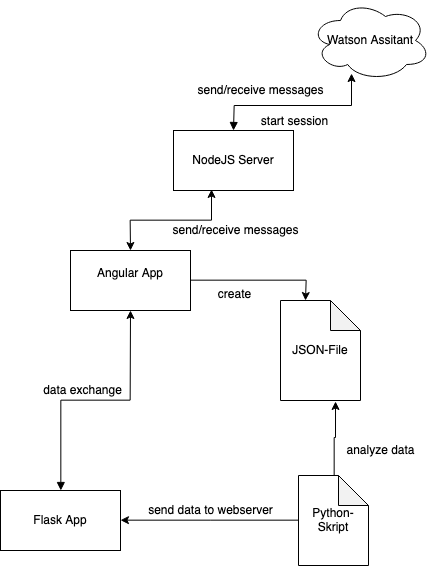
\includegraphics[width=1\textwidth]{images/architecture_perfectworld.png}
	\caption{Outlook: Architecture with Flask, Angular and Watson Assistant}
	\label{architecture_perfect}
\end{figure}

\chapter{Abbreviations}
\begin{acronym}[CRISP-DM]
\acro{crisp-dm}[CRISP-DM]{CRoss-Industry Standard Process for Data Mining}
\acro{cfo}[CFO]{Chief Financial Officer}
\acro{who}[WHO]{World Health Organization}
\acro{iarc}[IARC]{International Agency for Research on Cancer}
\acro{ham10000}[HAM10000]{Human Against Machine with 10000 training images}
\end{acronym}

\printbibliography[heading=bibintoc]

\chapter{Appendix A}\label{appendix a}
\ohead[]{Ehrenwörtliche Erklärung \hfill \thepage}

\null\vfill
\textbf{Ehrenwörtliche Erklärung}

Hiermit versichere ich, dass die vorliegende Arbeit von mir selbstständig und ohne unerlaubte Hilfe angefertigt worden ist, insbesondere dass ich alle Stellen, die wörtlich oder annähernd wörtlich aus Veröffentlichungen entnommen sind, durch Zitate als solche gekennzeichnet habe. Ich versichere auch, dass die von mir eingereichte schriftliche Version mit der digitalen Version übereinstimmt. Weiterhin erkläre ich, dass die Arbeit in gleicher oder ähnlicher Form noch keiner Prüfungsbehörde / Prüfungsstelle vorgelegen hat. Ich erkläre mich damit nicht einverstanden, dass die Arbeit der Öffentlichkeit zugänglich gemacht wird. Ich erkläre mich damit einverstanden, dass die Digitalversion dieser Arbeit zwecks Plagiatsprüfung auf die Server externer Anbieter hochgeladen werden darf. Die Plagiatsprüfung stellt keine Zurverfügungstellung für die Öffentlichkeit dar.

\ \\ \ \\ 


Ort, Datum (Vorname Nachname)

\vfill
\chapter{Appendix B}\label{appendix b}
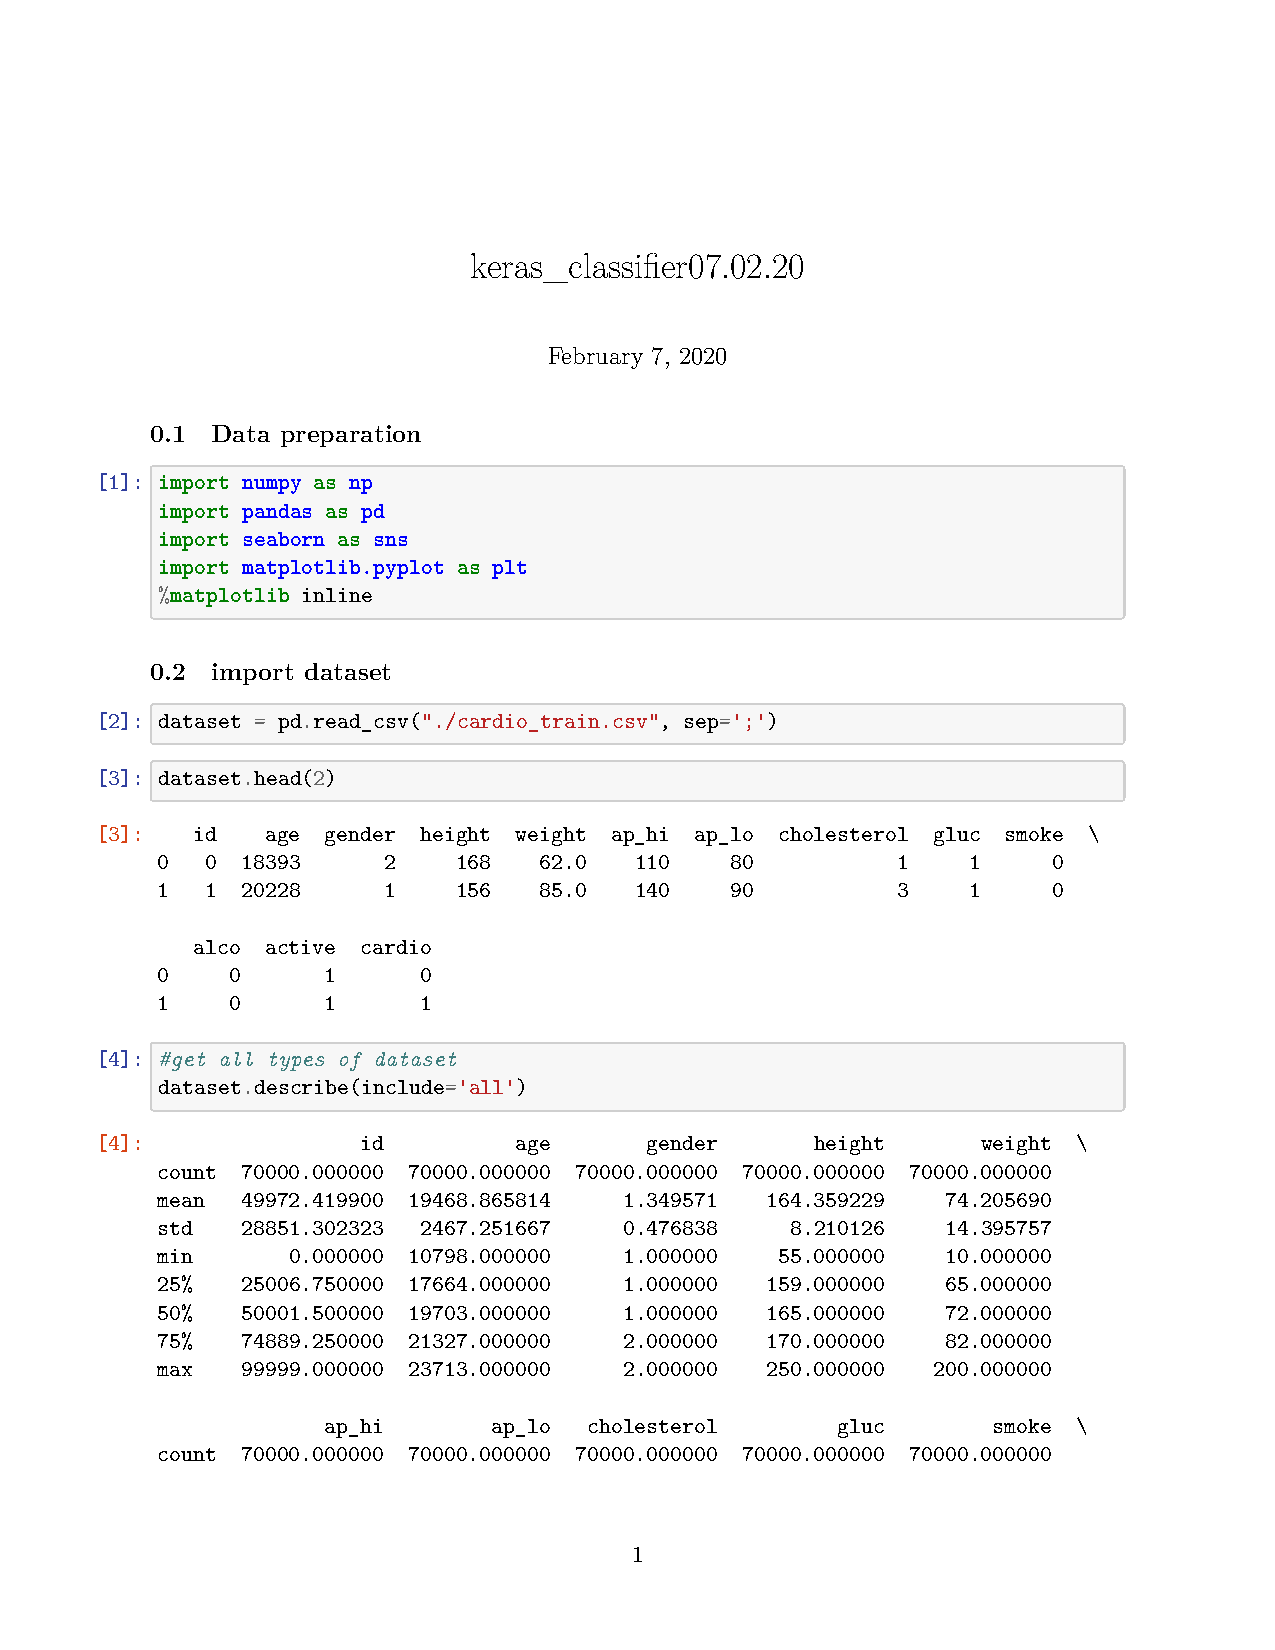
\includepdf[pages=-]{keras_classifier.pdf}

\end{document}
